% Options for packages loaded elsewhere
\PassOptionsToPackage{unicode}{hyperref}
\PassOptionsToPackage{hyphens}{url}
\documentclass[
]{article}
\usepackage{xcolor}
\usepackage{amsmath,amssymb}
\setcounter{secnumdepth}{5}
\usepackage{iftex}
\ifPDFTeX
  \usepackage[T1]{fontenc}
  \usepackage[utf8]{inputenc}
  \usepackage{textcomp} % provide euro and other symbols
\else % if luatex or xetex
  \usepackage{unicode-math} % this also loads fontspec
  \defaultfontfeatures{Scale=MatchLowercase}
  \defaultfontfeatures[\rmfamily]{Ligatures=TeX,Scale=1}
\fi
% \usepackage{lmodern}
\ifPDFTeX\else
  % xetex/luatex font selection
\fi
% Use upquote if available, for straight quotes in verbatim environments
\IfFileExists{upquote.sty}{\usepackage{upquote}}{}
\IfFileExists{microtype.sty}{% use microtype if available
  \usepackage[]{microtype}
  \UseMicrotypeSet[protrusion]{basicmath} % disable protrusion for tt fonts
}{}
\makeatletter
\@ifundefined{KOMAClassName}{% if non-KOMA class
  \IfFileExists{parskip.sty}{%
    \usepackage{parskip}
  }{% else
    \setlength{\parindent}{0pt}
    \setlength{\parskip}{6pt plus 2pt minus 1pt}}
}{% if KOMA class
  \KOMAoptions{parskip=half}}
\makeatother
\usepackage{longtable,booktabs,array}
\newcounter{none} % for unnumbered tables
\usepackage{calc} % for calculating minipage widths
% Correct order of tables after \paragraph or \subparagraph
\usepackage{etoolbox}
\makeatletter
\patchcmd\longtable{\par}{\if@noskipsec\mbox{}\fi\par}{}{}
\makeatother
% Allow footnotes in longtable head/foot
\IfFileExists{footnotehyper.sty}{\usepackage{footnotehyper}}{\usepackage{footnote}}
\makesavenoteenv{longtable}
\usepackage{graphicx}
\makeatletter
\newsavebox\pandoc@box
\newcommand*\pandocbounded[1]{% scales image to fit in text height/width
  \sbox\pandoc@box{#1}%
  \Gscale@div\@tempa{\textheight}{\dimexpr\ht\pandoc@box+\dp\pandoc@box\relax}%
  \Gscale@div\@tempb{\linewidth}{\wd\pandoc@box}%
  \ifdim\@tempb\p@<\@tempa\p@\let\@tempa\@tempb\fi% select the smaller of both
  \ifdim\@tempa\p@<\p@\scalebox{\@tempa}{\usebox\pandoc@box}%
  \else\usebox{\pandoc@box}%
  \fi%
}
% Set default figure placement to htbp
\def\fps@figure{htbp}
\makeatother
\setlength{\emergencystretch}{3em} % prevent overfull lines
\providecommand{\tightlist}{%
  \setlength{\itemsep}{0pt}\setlength{\parskip}{0pt}}
\usepackage[]{natbib}
\bibliographystyle{plainnat}
\makeatletter
\@ifpackageloaded{subcaption}{}{\usepackage{subcaption}}
\@ifpackageloaded{caption}{}{\usepackage{caption}}
\captionsetup[subfigure]{margin=0.5em}
\AtBeginDocument{%
\renewcommand*\figurename{Figure}
\renewcommand*\tablename{Table}
}
\AtBeginDocument{%
\renewcommand*\listfigurename{List of Figures}
\renewcommand*\listtablename{List of Tables}
}
\newcounter{pandoccrossref@subfigures@footnote@counter}
\newenvironment{pandoccrossrefsubfigures}{%
\setcounter{pandoccrossref@subfigures@footnote@counter}{0}
\begin{figure}\centering%
\gdef\global@pandoccrossref@subfigures@footnotes{}%
\DeclareRobustCommand{\footnote}[1]{\footnotemark%
\stepcounter{pandoccrossref@subfigures@footnote@counter}%
\ifx\global@pandoccrossref@subfigures@footnotes\empty%
\gdef\global@pandoccrossref@subfigures@footnotes{{##1}}%
\else%
\g@addto@macro\global@pandoccrossref@subfigures@footnotes{, {##1}}%
\fi}}%
{\end{figure}%
\addtocounter{footnote}{-\value{pandoccrossref@subfigures@footnote@counter}}
\@for\f:=\global@pandoccrossref@subfigures@footnotes\do{\stepcounter{footnote}\footnotetext{\f}}%
\gdef\global@pandoccrossref@subfigures@footnotes{}}
\@ifpackageloaded{float}{}{\usepackage{float}}
\floatstyle{ruled}
\@ifundefined{c@chapter}{\newfloat{codelisting}{h}{lop}}{\newfloat{codelisting}{h}{lop}[chapter]}
\floatname{codelisting}{Listing}
\newcommand*\listoflistings{\listof{codelisting}{List of Listings}}
\makeatother
\usepackage{bookmark}
\IfFileExists{xurl.sty}{\usepackage{xurl}}{} % add URL line breaks if available
\urlstyle{same}
% fallback for those not using the hyperref driver hyperxmp:
\makeatletter
\@ifundefined{xmpquote}{\newcommand{\xmpquote}[1]{#1}}{}
\makeatother
\hypersetup{
  colorlinks=true,linkcolor=red,urlcolor=red,citecolor=red,anchorcolor=red,filecolor=red,
  pdfcreator={LaTeX via pandoc}}

\author{}
\date{}

\IfFileExists{seqsplit.sty}{\usepackage{seqsplit}}{\newcommand{\seqsplit}[1]{#1}}
\protected\def\breakseq#1{\seqsplit{#1}}
\protected\def\breaktt#1{\begingroup\ttfamily\seqsplit{#1}\endgroup}
\title{Bounded AutoResearch for a Tiny Reproducible Machine-Learning Task}
\author{Daniel Ari Friedman\\\footnotesize{Active Inference Institute}\\\footnotesize{\texttt{daniel@activeinference.institute}}\\\footnotesize{\href{https://orcid.org/0000-0001-6232-9096}{ORCID: 0000-0001-6232-9096}} \\ \footnotesize{DOI: \href{https://doi.org/10.5281/zenodo.20417016}{10.5281/zenodo.20417016}}}
\date{\today}

\usepackage{geometry}
\geometry{margin=0.25in}
\usepackage{graphicx}
\usepackage{xcolor}

\begin{document}

\thispagestyle{empty}
\setlength{\parskip}{0pt}
\setlength{\itemsep}{0pt}
\begin{samepage}
\scriptsize

\section*{BEGINNING OF TRANSMISSION}\label{beginning-of-transmission}

\textbf{State:} published

\textbf{Pairing:} complete (DOI, GitHub, SHA-256, Zenodo URL)

\subsubsection*{Release metadata}

{\def\LTcaptype{none} % do not increment counter
\begin{longtable}[]{@{}
  >{\raggedright\arraybackslash}p{(\linewidth - 2\tabcolsep) * \real{0.5000}}
  >{\raggedright\arraybackslash}p{(\linewidth - 2\tabcolsep) * \real{0.5000}}@{}}
\toprule\noalign{}
\begin{minipage}[b]{\linewidth}\raggedright
Field
\end{minipage} & \begin{minipage}[b]{\linewidth}\raggedright
Value
\end{minipage} \\
\midrule\noalign{}
\endhead
\bottomrule\noalign{}
\endlastfoot
Title & Bounded AutoResearch for a Tiny Reproducible Machine-Learning
Task \\
Version & 0.3.2 \\
Concept DOI & 10.5281/zenodo.20417016 \\
Version DOI & 10.5281/zenodo.20931907 \\
GitHub &
\url{https://github.com/docxology/template_autoresearch_project/releases/tag/v0.3.2} \\
Zenodo & \url{https://zenodo.org/records/20417016} \\
SHA-256 & \breaktt{e07b62850a199593…} \\
SHA-512 & pending \\
\end{longtable}
}

\subsubsection*{How to verify}

\begin{itemize}
\tightlist
\item
  Scan \textbf{Integrity} QR and compare the embedded SHA-256 prefix to
  the table above.
\item
  Scan \textbf{Zenodo} / \textbf{GitHub} QR codes and confirm they
  resolve to this release pairing.
\item
  Full hashes and structured fields:
  \breaktt{../data/transmission\_manifest.json}.
\end{itemize}

\begin{figure}
\centering
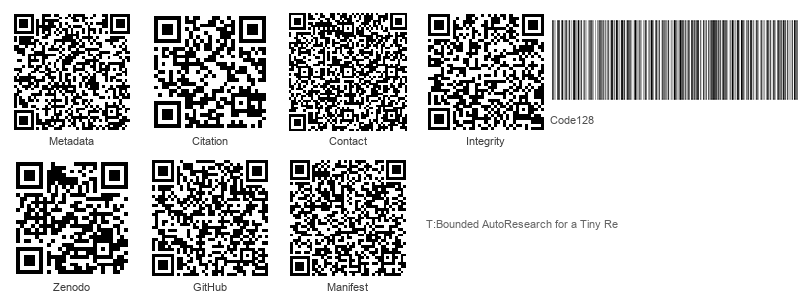
\includegraphics[width=0.98\linewidth,height=0.50\textheight,keepaspectratio,alt={Integrity QR strip}]{../figures/transmission_integrity_strip.png}
\caption{Integrity QR strip}
\end{figure}

Structured manifest: \breaktt{../data/transmission\_manifest.json}

\begin{figure}
\centering
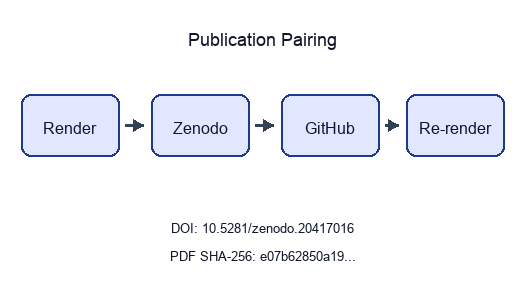
\includegraphics[width=0.35\linewidth,height=0.50\textheight,keepaspectratio,alt={Publication pairing flow}]{../figures/transmission_pairing.png}
\caption{Publication pairing flow}
\end{figure}

\textbf{Stego:} off |{} overlays text |{} barcodes on
|{} XMP on |{} manifest on \texorpdfstring{\ensuremath{\to}}{->} \texttt{./secure\_run.sh}

\end{samepage}
\newpage

\begin{titlepage}
\centering
\vspace*{2cm}
{\LARGE\bfseries Bounded AutoResearch for a Tiny Reproducible Machine-Learning Task\par}
\vspace{0.75em}
{\large A public exemplar for autoresearch, metric loops, evidence ledgers, review gates, and template orchestration\par}
\vfill
\makeatletter
{\@author\par}
\vspace{1em}
{\@date\par}
\makeatother
\vfill
\end{titlepage}
\thispagestyle{empty}
\newpage

\tableofcontents
\newpage


\newpage

\section{Abstract}\label{sec:abstract}

This paper presents
\breaktt{Deterministic\ bounded\ AutoResearch\ for\ a\ small\ MNIST\ neural-network\ task},
a public template exemplar that turns an AutoResearch loop into ordinary
reproducible research infrastructure. The case study is intentionally
small but concrete: \texttt{2000} training and \texttt{500} test images
from \breaktt{MNIST\ handwritten\ digit\ database} are evaluated by the
bounded \breaktt{small\ MNIST\ neural-network\ classification} loop. The
run evaluates \texttt{4} of \texttt{5} proposed candidates, including
\breaktt{Tiny\ patch-attention\ classifier}, selects
\texttt{exp-mlp-tanh-64} (\texttt{MLP}, \texttt{50890} parameters), and
improves \texttt{test\_accuracy} from \texttt{82.6\%} to \texttt{89.4\%}
(\texttt{6.8\%} absolute change). The validated diagnostic layer reports
macro F1 \texttt{89.4\%}, bootstrap accuracy interval
\breaktt{86.4\%\ to\ 92.0\%}, Brier score \texttt{0.161}, negative log
likelihood \texttt{0.361}, top-2 accuracy \texttt{95.6\%}, and exact
McNemar p-value \texttt{0.000}. The same pipeline writes proposal,
candidate, run, review, benchmark, evidence, figure, confusion-matrix,
statistical-summary, probability-quality, and security-integrity
artifacts from declared output contracts; uses \texttt{0} LLM calls at
USD \texttt{0.00} cost; and records \texttt{7} configured stages,
\texttt{6} supported local-artifact claims, and \texttt{78} required
artifacts. The local security attestation status is \texttt{passed},
with \texttt{0} checksum mismatch(es). The final readiness status is
\texttt{passed}, with review gates deferred to a human rather than
self-approved by the generated run.

\newpage

\section{Introduction}\label{sec:introduction}

\subsection{Bounded Research As
Infrastructure}\label{sec:bounded-research-infrastructure}

AutoResearch systems are most useful when their planning, evidence,
evaluation, and review surfaces remain inspectable. The recent pattern
popularized by bounded coding-agent research loops is simple: define a
tractable objective, try candidate changes under a budget, keep the
result that improves the metric, and leave a replayable trace of what
happened \citep{karpathy_autoresearch_2026}. That pattern is powerful,
but it is also easy to overstate. A public research template should show
how to run the loop without hiding cost, evidence, review, or execution
boundaries.

\subsection{Exemplar Task}\label{sec:exemplar-task}

This project implements that safer version. The central task is
\breaktt{small\ MNIST\ neural-network\ classification}:
\breaktt{MNIST\ handwritten\ digit\ database} from the handwritten-digit
database \citep{lecun_mnist_database}, a \breaktt{nearest-centroid}
baseline, and a finite list of candidate model families
(\breaktt{MLP,\ nearest-centroid,\ softmax\ regression,\ tiny\ patch-attention}).
The AutoResearch loop is responsible for proposing candidate
configurations, evaluating them against \texttt{test\_accuracy},
selecting the best result with deterministic tie-breaking, and writing
the evidence needed to review the claim.

\subsection{Contribution And Boundary}\label{sec:contribution-boundary}

The contribution is not a new \texttt{MNIST} classifier. It is a
template-level demonstration of how bounded AutoResearch can be
orchestrated through the same lifecycle used for reproducible papers:
tests run first, analysis writes structured artifacts, rendering
hydrates manuscript variables, validation checks evidence and readiness,
and copy stages publish final deliverables. The default path makes no
network calls, no LLM calls, executes no generated code, and never
treats a generated review packet as human approval. The methods in
sec.~\ref{sec:methodology} define that boundary, and the results in
sec.~\ref{sec:results} report only what the validated artifacts support.

\subsection{Process Organization
Motif}\label{sec:process-organization-motif}

The exemplar also treats research orchestration itself as a first-class
research object. In that limited operational sense, ``research for
research's sake'' means that programs, ledgers, evidence registries,
validation gates, and manuscript hydration do more than report a result:
they maintain the conditions under which the next research step can be
inspected, replayed, criticized, and extended. This is a process
analogy, not a moral claim that software is an end in itself or a
biological claim that the template is alive.

\subsection{Related Work And Current Trends}\label{sec:related-work}

\subsubsection{Information Overload And Machine-Readable
Science}\label{sec:information-overload-machine-readable-science}

The current AutoResearch literature is driven by a practical bottleneck:
scientific output is growing faster than document-centered review and
synthesis can absorb. Recent science-of-science evidence complicates any
simple productivity story: AI-augmented scientists can publish and be
cited more often, but the same adoption pattern can narrow the
collective range of topics and interactions in science
\citep{hao_ai_tools_focus_2026}. This is a 2026 Nature result, not a
2024 analysis, and it motivates governance rather than celebration.

One response is to make literature synthesis more source governed.
OpenScholar uses retrieval-augmented generation over a large scientific
passage store and reports citation accuracy improvements on literature
synthesis tasks \citep{asai_openscholar_2026}. PaperQA2 similarly
evaluates literature-search agents against expert scientific tasks and
emphasizes cited answers, contradiction detection, and factuality
\citep{skarlinski_paperqa2_2024}. STORM, PaperQA, and GPT Researcher are
adjacent source-grounded writing systems that motivate this project's
insistence on citation-backed claims and visible evidence surfaces
\citep{shao_storm_2024, lala_paperqa_2023, gpt_researcher_2026}. The
common lesson is that automated writing is not enough: claims must
remain tied to inspectable sources, artifacts, and evaluation records.

\subsubsection{Structured Distillation And Conceptual Knowledge
Substrates}\label{sec:structured-distillation-knowledge-substrates}

The Discovery Engine proposes a more structural answer to the same
overload problem. It distills publications into source-linked knowledge
artifacts, organizes those artifacts under a conceptual schema, encodes
them into a high-dimensional Conceptual Tensor, and unrolls that tensor
into graph and vector views for agent navigation
\citep{baulin_discovery_engine_2025}. This project does not construct a
Conceptual Nexus Model or claim domain-scale literature synthesis. It
adopts a much smaller analogue: outputs, ledgers, evidence registries,
figure records, and hydrated manuscript variables are file-backed
objects whose provenance can be checked before publication.

The representational background is broader than one framework. FAIR
principles argue for data that are findable, accessible, interoperable,
and reusable by people and machines \citep{wilkinson2016fair}. RO-Crate
and Workflow Run RO-Crate package research artifacts and computational
executions with linked-data metadata
\citep{soiland_reyes2022rocrate, soiland_reyes2024workflow_run_rocrate}.
Hyperdimensional computing and vector symbolic architectures provide one
route for robust high-dimensional symbolic-subsymbolic representations
\citep{heddes_hdc_2024}, while tensor factorization methods such as
TuckER and mixed-geometry tensor factorization show how multi-relational
knowledge graphs can be completed and queried as structured tensors
\citep{balazevic_tucker_2019, yusupov_mixed_geometry_2025}. The local
contribution here is not a new knowledge representation method; it is an
executable template that makes a small research workflow compatible with
that machine-readable direction.

\subsubsection{End-To-End AutoResearch
Systems}\label{sec:end-to-end-autoresearch-systems}

The most ambitious AutoResearch systems now aim at the entire scientific
lifecycle. The AI Scientist assembles idea generation, experiment
execution, paper writing, and automated review
\citep{lu_aiscientist_2024}, and its Nature version reports an
end-to-end AI research pipeline whose generated manuscript passed a
workshop peer-review round \citep{lu_ai_scientist_nature_2026}. AI
Scientist-v2 removes more hand-authored scaffolding and uses agentic
tree search for broader hypothesis exploration
\citep{yamada_ai_scientist_v2_2025}. FutureHouse's platform exposes
specialized scientific agents for literature search, deep review,
novelty checking, and chemistry planning
\citep{futurehouse_platform_2025}, while Robin integrates literature and
data-analysis agents in a lab-in-the-loop discovery workflow
\citep{ghareeb_robin_2026}.

Survey work is already separating reliable assistance from risky
autonomy. The AI for Auto-Research roadmap describes the full lifecycle
from creation to dissemination, but stresses that novelty,
research-level implementation, and judgment remain fragile under
automation \citep{kong_ai_auto_research_2026}. EXHYTE frames discovery
as an iterative Exploration, Hypothesis generation, and Testing loop,
clarifying where current systems are mature and where closed-loop
autonomy remains thin \citep{hasib_exhyte_2025}. This exemplar therefore
takes the opposite stance from full autonomy: it implements a bounded
local loop whose candidate space, data, cost, outputs, and review gates
can be audited.

\subsubsection{Autoformalization And
Verification}\label{sec:autoformalization-verification}

Autoformalization supplies a different kind of boundary: instead of only
asking whether generated text is plausible, it asks whether an informal
statement can be translated into a form that a proof assistant or
compiler can check. AlphaProof shows the power of reinforcement learning
over formal mathematical proof search \citep{hubert_alphaproof_2025}.
Process-driven autoformalization in Lean uses compiler feedback as a
precise signal for improving translations from natural-language
mathematics to formal statements and proofs
\citep{lu_process_driven_autoformalization_2024}. APOLLO turns Lean
feedback into an iterative proof-repair workflow in which generated
proofs are decomposed, patched, and reverified
\citep{apollo_lean_collaboration_2025}.

This project does not perform theorem proving, proof repair, or formal
mathematical verification. It borrows the architectural lesson:
generated research artifacts should be checked by deterministic tools
with explicit error surfaces. Here those tools are test suites, schema
checks, evidence registries, render validation, source hygiene greps,
and review packets rather than Lean, Isabelle, or Coq.

\subsubsection{ML For ML And Evolutionary Algorithm
Discovery}\label{sec:ml-for-ml-evolutionary-discovery}

ML-for-ML systems optimize models, code, or algorithms with search loops
that are themselves subject to evaluation. Karpathy's
\texttt{autoresearch} repository frames a minimal version of this
pattern as a prompt-controlled system with a fixed budget, editable code
surface, and comparable metric \citep{karpathy_autoresearch_2026}.
MLAgentBench and MLE-bench package machine learning tasks as scored,
replayable environments with logs and grading outputs
\citep{huang_mlagentbench_2023, chan_mle_bench_2024}.

At a larger scale, AlphaEvolve couples language-model proposals to
evolutionary program search and automated evaluators, producing
algorithmic improvements in mathematics and computing
\citep{romera_paredes_alphaevolve_2025}. DeepEvolve adds external
retrieval, multi-file code editing, and debugging to the same basic
proposal-implementation-evaluation loop \citep{deepevolve_2025}. This
manuscript's candidate search is intentionally smaller: a finite list of
configured model families is evaluated against \texttt{test\_accuracy},
with deterministic selection and recorded deferrals rather than
unbounded code mutation.

\subsubsection{Agentic Science, Graph Retrieval, And Epistemic
Foraging}\label{sec:agentic-science-graph-retrieval}

Agentic science surveys describe systems that move from tool use toward
scientific agency across perception, knowledge representation, planning,
experimentation, analysis, and communication
\citep{wei_agentic_science_2025, gridach_agentic_science_2025}. GraphRAG
work adds structured retrieval to that picture: graph construction and
graph-aware retrieval can support multi-hop reasoning, but benchmarks
also show that knowledge-graph RAG remains brittle when relevant
knowledge is incomplete \citep{graphrag_bench_2026, brink_kg_rag_2026}.
Active-inference perspectives make a similar design demand in different
language: scientific agents need persistent uncertainty-aware memory,
causal models, counterfactual exploration, deterministic validation, and
human judgment as an architectural component
\citep{active_inference_science_2025}.

This exemplar uses those ideas as constraints, not as capabilities it
already possesses. It does not run live literature mining, autonomous
proof search, external agent swarms, graph-based hypothesis hunting, or
self-approval. Instead it exposes bounded candidates, explicit budgets,
local evidence links, local \texttt{MNIST} input data, benchmark-style
scoring, source-linked figures, manuscript hydration, and human review
gates. That is the intended safe baseline for a public template.

\subsubsection{Benchmark, Documentation, And Process
Analogies}\label{sec:benchmark-documentation-process-analogies}

\texttt{MNIST} and LeNet remain useful here because they provide a
compact historical benchmark for small neural networks and handwriting
recognition \citep{lecun_gradient_1998, lecun_mnist_database}. Vision
Transformers introduce the patch-token pattern for image classification
at scale \citep{dosovitskiy_vit_2020}; this exemplar borrows only the
patching and attention representation through
\breaktt{Tiny\ patch-attention\ classifier}, then keeps the
implementation inside the configured candidate budget. MLPerf Tiny and
OpenML motivate explicit task descriptions, fixed inputs,
machine-readable run metadata, and checkable metrics
\citep{banbury_mlperf_tiny_2021, vanschoren_openml_2014}.
Machine-learning reproducibility checklists motivate reporting data,
seeds, model sizes, hyperparameters, and compute boundaries
\citep{pineau_reproducibility_2020}.

Dataset and model documentation work further informs the safe boundary.
Datasheets for Datasets motivate explicit reporting of dataset
motivation, composition, collection, and recommended use
\citep{gebru2021datasheets}. Model Cards motivate structured reporting
of model context, intended use, evaluation procedure, and limitations
\citep{mitchell2019model_cards}. The diagnostic layer follows the same
conservative reporting posture: calibration is treated as separate from
accuracy \citep{guo2017calibration}, binomial accuracy intervals use
Wilson-style score intervals \citep{wilson1927probable_inference},
matched classifier comparison is summarized through paired discordance
\citep{dietterich1998statistical_tests}, deterministic bootstrap
intervals are local resampling diagnostics \citep{efron1993bootstrap},
and probability quality is reported with Brier score, negative log
likelihood, and chance-corrected agreement
\citep{brier1950verification, cohen1960coefficient}.

The process language is borrowed cautiously from teleology and
theoretical biology. Kant's account of organized beings treats a natural
purpose as a whole whose parts and whole mutually condition one another
\citep{ginsborg_kant_aesthetics_teleology}. Autopoiesis characterizes
living systems through self-producing organization
\citep{varela_autopoiesis_1974}, and later work connects Kantian natural
purpose to autopoietic individuality
\citep{weber_varela_life_after_kant_2002}. Moreno and Mossio's account
of biological autonomy emphasizes organizational closure and
self-maintenance \citep{moreno_mossio_biological_autonomy_2015}. This
paper uses those ideas only as disciplined analogies for configured
scientific workflows whose artifacts help reproduce, constrain, and
evaluate subsequent artifacts.

Security and supply-chain references enter with the same restraint.
NIST's zero-trust architecture treats verification as explicit and
continuous rather than inherited from a trusted perimeter
\citep{nist_sp800_207_zero_trust}. The NIST Secure Software Development
Framework emphasizes repeatable practices for reducing software
vulnerability risk \citep{nist_sp800_218_ssdf}. SLSA frames
software-artifact provenance and supply-chain integrity as a graded
assurance problem \citep{slsa_spec_latest}, while MITRE ATT\&CK T1195
names supply-chain compromise as a concrete adversary technique
\citep{mitre_attack_t1195}. This exemplar borrows those frameworks as
disciplined analogies for local research artifact integrity: checksums,
inventories, review gates, and explicit non-claims, not production
deployment certification.

\newpage

\section{Methodology}\label{sec:methodology}

The loop is implemented through the project source surface summarized by
the validated run artifacts. The project scripts remain thin
dispatchers; reusable behavior writes
\breaktt{output/data/autoresearch\_loop.json},
\breaktt{output/data/ml\_task\_results.json},
\breaktt{../figures/figure\_registry.json},
\breaktt{output/data/autoresearch\_phase\_ledger.json}, and
\breaktt{output/data/manuscript\_variable\_provenance.json}.

\subsection{Task And Data}\label{sec:task-data}

The task is \breaktt{small\ MNIST\ neural-network\ classification}. The
default configuration loads \breaktt{data/mnist\_small.npz}, with
provenance in \breaktt{data/mnist\_small\_provenance.json}, and uses seed
\texttt{20260525}. The subset contains \texttt{2000} training images and
\texttt{500} test images, with \texttt{10} classes present in both
splits and image shape \texttt{28\ by\ 28}. The provenance artifact
records upstream source-file hashes, the subset seed, class counts, and
the compressed subset hash. The default pipeline never downloads data at
runtime. The train and test splits contain \texttt{200} and \texttt{50}
examples per class, respectively. The registered class-balance
diagnostic is fig.~\ref{fig:mnist_class_balance}, and the dataset
contact sheet is fig.~\ref{fig:mnist_subset_contact_sheet}.

\begin{figure}
\centering
\pandocbounded{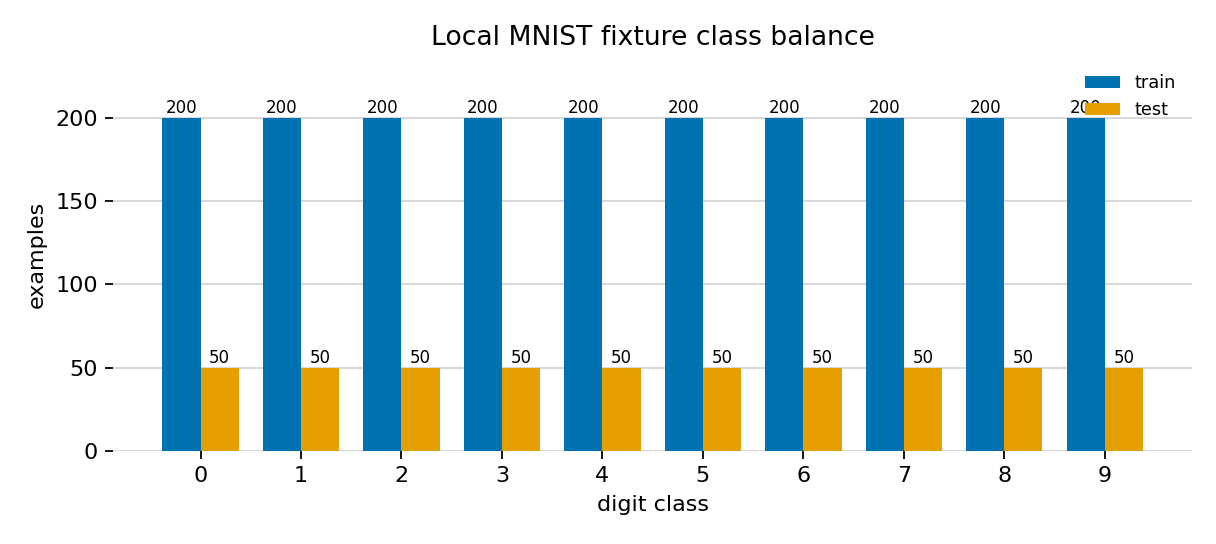
\includegraphics[keepaspectratio,alt={Train and test class counts from output/data/ml\_class\_balance.json; the local fixture contains 2000 train and 500 test examples across 10 classes. Generation method: Grouped train/test class-count bars from the local MNIST fixture. Registry metadata records the generation method, source artifact, and claim boundary for validation.}]{../figures/mnist_class_balance.png}}
\caption{Train and test class counts from
output/data/ml\_class\_balance.json; the local fixture contains 2000
train and 500 test examples across 10 classes. Generation method:
Grouped train/test class-count bars from the local MNIST fixture.
Registry metadata records the generation method, source artifact, and
claim boundary for validation.}\label{fig:mnist_class_balance}
\end{figure}

\begin{longtable}[]{@{}llll@{}}
\caption{Local fixture class-balance table from
\protect\breaktt{output/data/ml\_class\_balance.json}; counts describe
the offline fixture used by this
run.}\label{tbl:class-balance}\tabularnewline
\toprule\noalign{}
Split & Class & Count & Fraction \\
\midrule\noalign{}
\endfirsthead
\toprule\noalign{}
Split & Class & Count & Fraction \\
\midrule\noalign{}
\endhead
\bottomrule\noalign{}
\endlastfoot
train & 0 & 200 & 10.0\% \\
train & 1 & 200 & 10.0\% \\
train & 2 & 200 & 10.0\% \\
train & 3 & 200 & 10.0\% \\
train & 4 & 200 & 10.0\% \\
train & 5 & 200 & 10.0\% \\
train & 6 & 200 & 10.0\% \\
train & 7 & 200 & 10.0\% \\
train & 8 & 200 & 10.0\% \\
train & 9 & 200 & 10.0\% \\
test & 0 & 50 & 10.0\% \\
test & 1 & 50 & 10.0\% \\
test & 2 & 50 & 10.0\% \\
test & 3 & 50 & 10.0\% \\
test & 4 & 50 & 10.0\% \\
test & 5 & 50 & 10.0\% \\
test & 6 & 50 & 10.0\% \\
test & 7 & 50 & 10.0\% \\
test & 8 & 50 & 10.0\% \\
test & 9 & 50 & 10.0\% \\
\end{longtable}

\begin{figure}
\centering
\pandocbounded{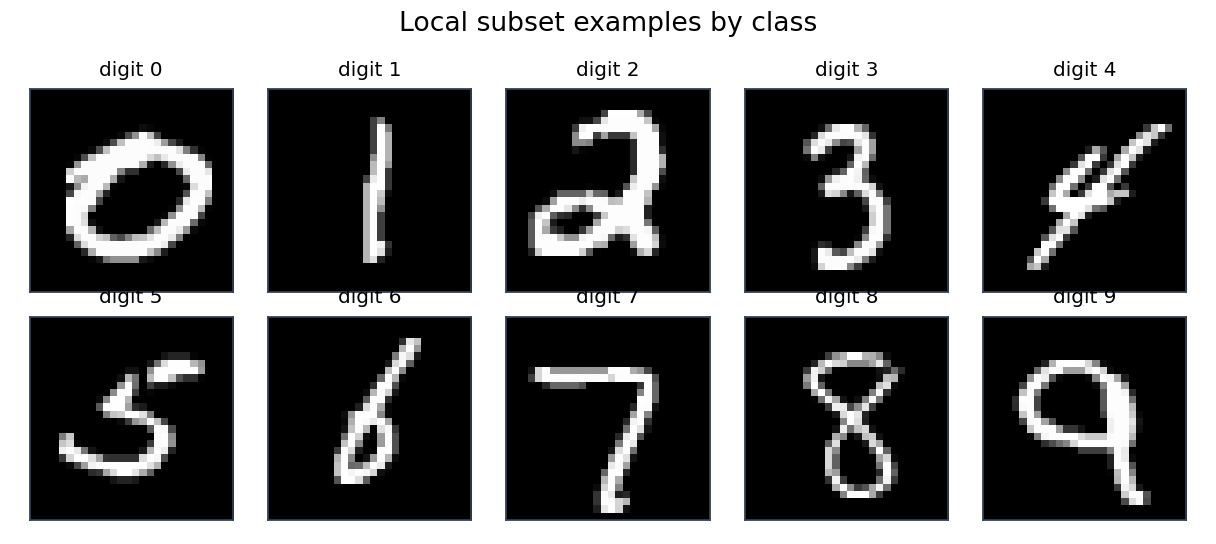
\includegraphics[keepaspectratio,alt={Deterministic class-balanced contact sheet for MNIST handwritten digit database from data/mnist\_small.npz and data/mnist\_small\_provenance.json; the figure documents the local subset used by the offline run. Generation method: Class-balanced contact sheet from fixed local MNIST arrays. Registry metadata records the generation method, source artifact, and claim boundary for validation.}]{../figures/mnist_subset_contact_sheet.png}}
\caption{Deterministic class-balanced contact sheet for MNIST
handwritten digit database from data/mnist\_small.npz and
data/mnist\_small\_provenance.json; the figure documents the local
subset used by the offline run. Generation method: Class-balanced
contact sheet from fixed local MNIST arrays. Registry metadata records
the generation method, source artifact, and claim boundary for
validation.}\label{fig:mnist_subset_contact_sheet}
\end{figure}

The baseline is \breaktt{nearest\_centroid\_baseline}
(\breaktt{nearest-centroid}). The bounded candidate set is configured by
the task artifact and covers
\breaktt{MLP,\ nearest-centroid,\ softmax\ regression,\ tiny\ patch-attention},
including \breaktt{Tiny\ patch-attention\ classifier} and at least one
deferred proposal. The transformer-style candidate borrows the
patch-token representation for comparison while staying inside the
configured iteration budget. This is intentionally a small configured
model, not a claim about full-scale image-transformer performance.

\subsection{Bounded Loop}\label{sec:bounded-loop}

The run follows \texttt{7} configured stages:

\begin{itemize}
\tightlist
\item
  Resolve the human-authored program, project topic, and research
  questions.
\item
  Build an \breaktt{AutoResearchPlan} from the domain profile, experiment
  plan, and pipeline DAG.
\item
  Validate exact stage-gate names declared in
  \breaktt{autoresearch.yaml}.
\item
  Evaluate the configured \texttt{MNIST} candidate set up to the
  configured iteration budget.
\item
  Generate claims only from configured questions and local artifact
  paths.
\item
  Write data, reports, figures, benchmark scores, and review packets
  under the declared output contract.
\item
  Run strict AutoResearch readiness validation and write readiness
  reports.
\end{itemize}

Candidates are declared in the proposal ledger and resolved from the
task configuration for execution. Each executable candidate declares a
model type, seed, training schedule, and model-specific parameters. The
configured training policy includes learning-rate decay \texttt{0.995}
and gradient clipping norm \texttt{5}, both recorded from the validated
task run rather than described as a free-form manuscript setting. The
loop evaluates at most \texttt{4} configured iterations, selects the
highest \texttt{test\_accuracy}, and breaks ties by lower parameter
count and identifier. Candidates outside the budget are recorded as
deferred; the run-derived status summary is
\breaktt{accepted:\ 1,\ deferred:\ 1,\ rejected:\ 3}.

The closure is concrete and file-backed.
\breaktt{output/data/research\_program.json} constrains proposals;
proposal records feed the bounded evaluation; evaluation writes
\breaktt{output/data/ml\_candidate\_ledger.json} and
\breaktt{output/data/run\_ledger.json}; ledgers support artifact-linked
claims; claims hydrate the manuscript through
\breaktt{output/data/manuscript\_variables.json}; readiness validation
writes \breaktt{output/reports/autoresearch\_readiness.json}; loop
settlement is recorded in
\breaktt{output/data/autoresearch\_phase\_ledger.json}; and review state
is captured in \breaktt{output/data/review\_decisions.json}. The loop
therefore maintains an inspectable research process around a small
metric result without making the process self-approving or opaque.

The concrete closure is intentionally close to research-object and
workflow-run provenance practice. The artifact manifest lists generated
objects and checksums; the figure registry binds captions to source
artifacts; the variable provenance sidecar records the source pointer
for each injected token or table; and the review packet keeps human
decisions outside generated approval. This is a minimal local analogue
of machine-readable provenance rather than a claim of full
research-object packaging.

The generated schema manifest at
\breaktt{output/data/autoresearch\_schema\_manifest.json} records
\texttt{31} schema-versioned governance payload(s) plus documented
generic-table exemptions. The local research-object manifest at
\breaktt{output/data/research\_object\_manifest.json} packages observed
project paths, hashes, the evidence registry, the source ledger, the
schema manifest, and the manual approval state. It is deliberately named
a local research-object manifest, not RO-Crate or SLSA compliance.

\subsection{Safety Controls}\label{sec:safety-controls}

The default autonomy level is \texttt{proposal\_only}. The run ledger
records \texttt{0} LLM calls and USD \texttt{0.00} cost. The edit
allowlist is restricted to the public project source and manuscript
surfaces, plus the task configuration file, and the pipeline never
executes generated code. Review gates are emitted with deferred
decisions so that validation can confirm the gates exist without
pretending that the machine approved publication.

Publication approval is a non-generated input. The run may read
\breaktt{human\_review.yaml} and copy its state into review payloads, but
generated readiness cannot set publication approval by itself; the
default local review state remains \texttt{false}.

Disclosure: \breaktt{AI-assisted\ AutoResearch} status is declared for
this exemplar because it models machine-produced plans, ledgers,
reports, and manuscript variables as review inputs rather than
autonomous approval.

\subsection{Adversarial And Supply-Chain
Controls}\label{sec:adversarial-supply-chain-controls}

The security layer is configured as \breaktt{local\_deterministic} with
network policy \texttt{default\_offline}, integrity algorithm
\texttt{sha256}, external signing \texttt{false}, and framework labels
\breaktt{STRIDE,\ MITRE\_ATT\&CK\_T1195}. Its scope is
\breaktt{Local\ research-artifact\ integrity\ evidence\ for\ this\ deterministic\ public\ exemplar}.
These values are generated from
\breaktt{output/data/autoresearch\_security\_profile.json}; the default
run remains offline and deterministic.

The local threat model covers \texttt{7} asset(s), \texttt{7} threat
row(s), and \texttt{7} control row(s). The security artifacts are
written to \breaktt{output/data/autoresearch\_threat\_model.json},
\breaktt{output/data/autoresearch\_supply\_chain\_inventory.json},
\breaktt{output/data/autoresearch\_integrity\_attestation.json}, and
\breaktt{output/reports/autoresearch\_security\_review.md}. The
control-matrix figure is
fig.~\ref{fig:autoresearch_security_control_matrix}. The table and
figure are generated from the threat model and inventory, not manually
maintained.

\begin{figure}
\centering
\pandocbounded{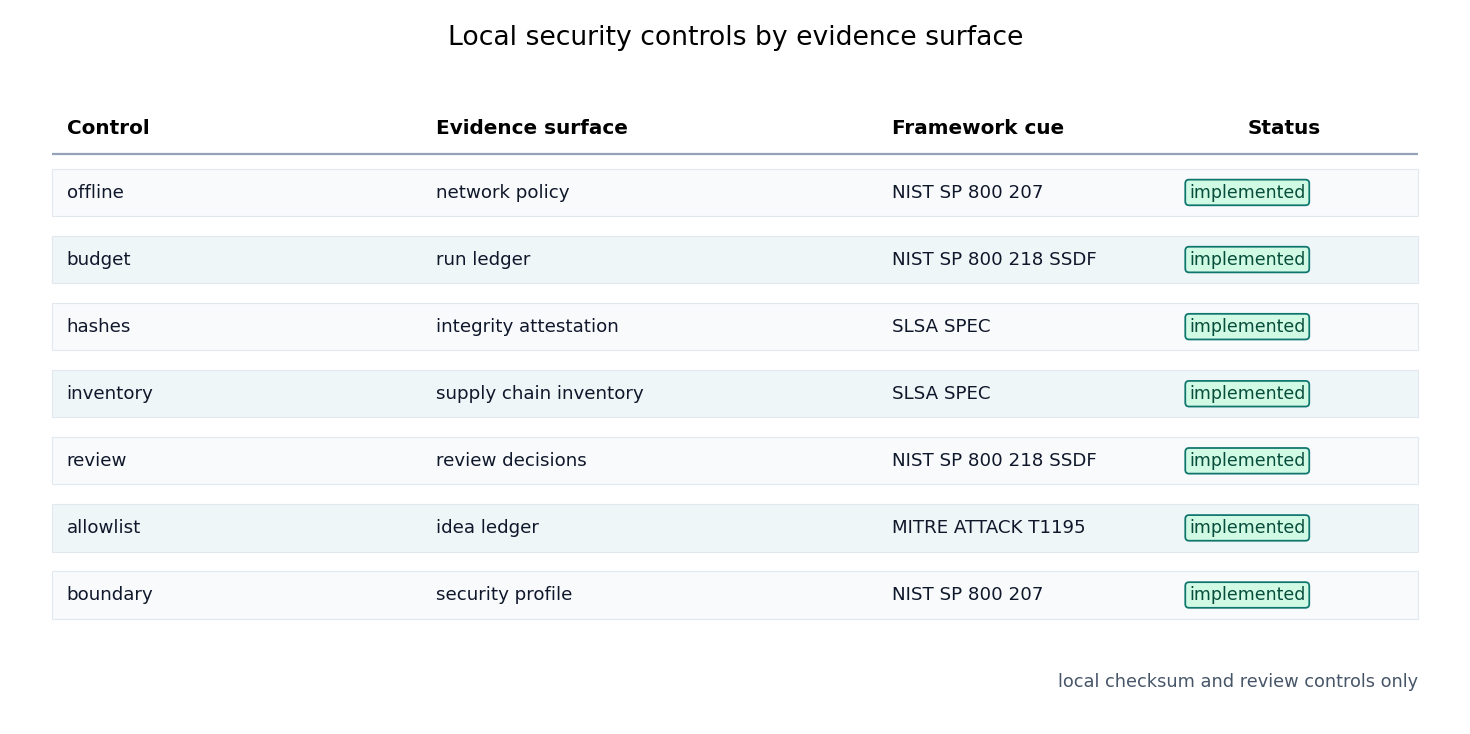
\includegraphics[keepaspectratio,alt={Local security-control matrix from output/data/autoresearch\_threat\_model.json; controls map NIST, SLSA, and ATT\&CK-inspired safeguards to deterministic evidence surfaces without claiming production security certification. Generation method: structured control matrix with separate control, evidence, framework, and status columns. Generation method: Structured control matrix from local threat-model controls. Registry metadata records the generation method, source artifact, and claim boundary for validation.}]{../figures/autoresearch_security_control_matrix.png}}
\caption{Local security-control matrix from
output/data/autoresearch\_threat\_model.json; controls map NIST, SLSA,
and ATT\&CK-inspired safeguards to deterministic evidence surfaces
without claiming production security certification. Generation method:
structured control matrix with separate control, evidence, framework,
and status columns. Generation method: Structured control matrix from
local threat-model controls. Registry metadata records the generation
method, source artifact, and claim boundary for
validation.}\label{fig:autoresearch_security_control_matrix}
\end{figure}

\begin{longtable}[]{@{}
  >{\raggedright\arraybackslash}p{(\linewidth - 4\tabcolsep) * \real{0.3333}}
  >{\raggedright\arraybackslash}p{(\linewidth - 4\tabcolsep) * \real{0.3333}}
  >{\raggedright\arraybackslash}p{(\linewidth - 4\tabcolsep) * \real{0.3333}}@{}}
\caption{Local security artifacts generated for the bounded AutoResearch
run.}\label{tbl:security-artifacts}\tabularnewline
\toprule\noalign{}
\begin{minipage}[b]{\linewidth}\raggedright
Security artifact
\end{minipage} & \begin{minipage}[b]{\linewidth}\raggedright
Path
\end{minipage} & \begin{minipage}[b]{\linewidth}\raggedright
Summary
\end{minipage} \\
\midrule\noalign{}
\endfirsthead
\toprule\noalign{}
\begin{minipage}[b]{\linewidth}\raggedright
Security artifact
\end{minipage} & \begin{minipage}[b]{\linewidth}\raggedright
Path
\end{minipage} & \begin{minipage}[b]{\linewidth}\raggedright
Summary
\end{minipage} \\
\midrule\noalign{}
\endhead
\bottomrule\noalign{}
\endlastfoot
profile & \href{../data/autoresearch_security_profile.json}{security
profile} & local\_deterministic \\
threat model & \href{../data/autoresearch_threat_model.json}{threat
model} & default\_offline \\
inventory &
\href{../data/autoresearch_supply_chain_inventory.json}{supply
inventory} & 14 inputs \\
inventory export &
\href{../data/autoresearch_inventory_export.json}{inventory export} &
local non-SBOM export \\
attestation &
\href{../data/autoresearch_integrity_attestation.json}{integrity
attestation} & passed \\
review & \href{../reports/autoresearch_security_review.md}{security
review} & human review input \\
\end{longtable}

\begingroup\footnotesize

\begin{longtable}[]{@{}
  >{\raggedright\arraybackslash}p{(\linewidth - 8\tabcolsep) * \real{0.2000}}
  >{\raggedright\arraybackslash}p{(\linewidth - 8\tabcolsep) * \real{0.2000}}
  >{\raggedright\arraybackslash}p{(\linewidth - 8\tabcolsep) * \real{0.2000}}
  >{\raggedright\arraybackslash}p{(\linewidth - 8\tabcolsep) * \real{0.2000}}
  >{\raggedright\arraybackslash}p{(\linewidth - 8\tabcolsep) * \real{0.2000}}@{}}
\caption{Threat-model rows from
\protect\breaktt{output/data/autoresearch\_threat\_model.json}; ATT\&CK
labels scope supply-chain compromise
analogies.}\label{tbl:security-threat-model}\tabularnewline
\toprule\noalign{}
\begin{minipage}[b]{\linewidth}\raggedright
Threat
\end{minipage} & \begin{minipage}[b]{\linewidth}\raggedright
STRIDE
\end{minipage} & \begin{minipage}[b]{\linewidth}\raggedright
ATT\&CK
\end{minipage} & \begin{minipage}[b]{\linewidth}\raggedright
Scenario
\end{minipage} & \begin{minipage}[b]{\linewidth}\raggedright
Residual risk
\end{minipage} \\
\midrule\noalign{}
\endfirsthead
\toprule\noalign{}
\begin{minipage}[b]{\linewidth}\raggedright
Threat
\end{minipage} & \begin{minipage}[b]{\linewidth}\raggedright
STRIDE
\end{minipage} & \begin{minipage}[b]{\linewidth}\raggedright
ATT\&CK
\end{minipage} & \begin{minipage}[b]{\linewidth}\raggedright
Scenario
\end{minipage} & \begin{minipage}[b]{\linewidth}\raggedright
Residual risk
\end{minipage} \\
\midrule\noalign{}
\endhead
\bottomrule\noalign{}
\endlastfoot
dataset tamper & Tampering & T1195 & A local fixture could be replaced
or edited before analysis. & Residual risk remains if a reviewer ignores
checksum drift. \\
config drift & Tampering & T1195.001 & Task settings could silently
change candidate scope, budgets, or diag\ldots{} & Configuration review
is still a human responsibility. \\
source edit & Elevation of privilege & T1195.001 & Source changes could
bypass the thin-script and no-generated-code bou\ldots{} & The default
run does not perform full static application security tes\ldots{} \\
output tamper & Repudiation & T1195.002 & Generated reports or figures
could be edited after analysis but befor\ldots{} & Local checksum
evidence is not externally signed. \\
manuscript injection & Information disclosure & T1195.002 & Manual prose
could hard-code run facts that bypass validated variables. & Stable
scholarly prose and citekeys remain manually authored. \\
self approval & Spoofing & T1195 & Generated review packets could be
mistaken for human publication appr\ldots{} & Publication remains
outside the automated loop. \\
build assumption & Denial of service & T1195.003 & A local or CI build
context could omit checks or run stale generated\ldots{} & The exemplar
does not sign build logs or isolate runners. \\
\end{longtable}

\endgroup

\subsection{Positioning Against Autonomous Science
Systems}\label{sec:positioning-autonomous-science}

The implementation should be read as a bounded local analogue of current
AutoResearch trends, not as a miniature autonomous scientist. Artifact
manifests, evidence registries, review gates, and manuscript hydration
provide machine-readable governance surfaces for one offline project
run. They do not perform autonomous literature mining, proof search,
live agent orchestration, runtime dataset expansion, self-modifying code
search, or self-approval of publication claims.

\subsection{Evidence And Scoring}\label{sec:evidence-scoring}

The experiment writes \breaktt{output/data/ml\_task\_results.json},
\breaktt{output/data/ml\_candidate\_ledger.json},
\breaktt{output/data/ml\_confusion\_matrix.csv},
\breaktt{output/data/ml\_training\_history.csv},
\breaktt{output/data/ml\_error\_examples.json},
\breaktt{output/data/ml\_prediction\_records.json},
\breaktt{output/data/ml\_classification\_diagnostics.json},
\breaktt{output/data/ml\_candidate\_intervals.json},
\breaktt{output/data/ml\_class\_balance.json},
\breaktt{output/data/ml\_calibration\_report.json},
\breaktt{output/data/ml\_calibration\_bin\_intervals.json},
\breaktt{output/data/ml\_robustness\_report.json},
\breaktt{output/data/ml\_probability\_diagnostics.json},
\breaktt{output/data/ml\_bootstrap\_intervals.json},
\breaktt{output/data/ml\_paired\_comparison.json},
\breaktt{output/data/ml\_candidate\_rank\_stability.json},
\breaktt{output/data/ml\_statistical\_summary.json},
\breaktt{output/data/ml\_training\_diagnostics.json},
\breaktt{output/reports/ml\_benchmark\_score.json},
\breaktt{output/data/benchmark\_boundary.json},
\breaktt{output/data/figure\_quality\_report.json}, and registered
figures through \breaktt{../figures/figure\_registry.json}. The
diagnostic payloads preserve probabilities, confidence and margin
summaries, class metrics, calibration bins, confusion-pair summaries,
train/test gaps, deterministic no-retrain perturbation scores, bootstrap
intervals, paired baseline comparison, rank-stability frequencies,
calibration-bin Wilson intervals, selective accuracy thresholds, Brier
score, negative log likelihood, top-2 accuracy, probability-quality
comparisons, learning-rate traces, best-epoch markers, final learning
rates, and train-test gap summaries without serializing model weights.
The benchmark score combines metric improvement, budget compliance,
offline execution, transformer-candidate coverage, and
candidate-selection status. The benchmark-boundary artifact records
fixture scope, metric direction, candidate families, budget,
statistical-method artifacts, and explicit non-claims, so
benchmark-adjacent statistics remain local readiness diagnostics rather
than broad empirical or publication claims. Manuscript variables are
hydrated from these artifacts, and readiness validation checks
\breaktt{output/reports/evidence\_registry.json},
\breaktt{output/reports/artifact\_manifest.json}, method ledgers, review
gates, benchmark outputs, the phase ledger, figure-quality report, and
AI-assisted disclosure before rendering is treated as ready for review.
The reviewer-facing
\breaktt{output/data/autoresearch\_evidence\_overview.json} then
summarizes readiness versus publication approval, claim-evidence rows,
source-ledger status, benchmark boundary issues, and security/integrity
status without granting approval. The generated tables and figure blocks
used in sec.~\ref{sec:results} are sourced through
\breaktt{output/data/manuscript\_variable\_provenance.json} and
\breaktt{output/data/manuscript\_figure\_blocks.json}, so captions,
artifact tables, and run-derived result statements share the same
validated artifact base.

The figure registry also carries the method contract for each
visualization: source artifact, generated file, rendering method, and
claim boundary. The rendered method table below is generated from that
registry rather than maintained manually.

\begingroup\footnotesize

\begin{longtable}[]{@{}
  >{\raggedright\arraybackslash}p{(\linewidth - 6\tabcolsep) * \real{0.2500}}
  >{\raggedright\arraybackslash}p{(\linewidth - 6\tabcolsep) * \real{0.2500}}
  >{\raggedright\arraybackslash}p{(\linewidth - 6\tabcolsep) * \real{0.2500}}
  >{\raggedright\arraybackslash}p{(\linewidth - 6\tabcolsep) * \real{0.2500}}@{}}
\caption{Registry-backed figure methods from
\href{../figures/figure_registry.json}{\protect\breaktt{figure\_registry.json}};
full validation hooks, alt text, and claim boundaries remain in the
registry.}\label{tbl:figure-methods}\tabularnewline
\toprule\noalign{}
\begin{minipage}[b]{\linewidth}\raggedright
Figure
\end{minipage} & \begin{minipage}[b]{\linewidth}\raggedright
Source
\end{minipage} & \begin{minipage}[b]{\linewidth}\raggedright
Method
\end{minipage} & \begin{minipage}[b]{\linewidth}\raggedright
Scope
\end{minipage} \\
\midrule\noalign{}
\endfirsthead
\toprule\noalign{}
\begin{minipage}[b]{\linewidth}\raggedright
Figure
\end{minipage} & \begin{minipage}[b]{\linewidth}\raggedright
Source
\end{minipage} & \begin{minipage}[b]{\linewidth}\raggedright
Method
\end{minipage} & \begin{minipage}[b]{\linewidth}\raggedright
Scope
\end{minipage} \\
\midrule\noalign{}
\endhead
\bottomrule\noalign{}
\endlastfoot
fig.~\ref{fig:autoresearch_candidate_lifecycle} &
\href{../data/ml_candidate_ledger.json}{candidate ledger} & Candidate
lifecycle status-count bar chart. & Lifecycle counts describe bounded
orchestration, not autonomous approval. \\
fig.~\ref{fig:autoresearch_closure_flow} &
\href{../data/autoresearch_loop.json}{loop} & File-backed process-flow
diagram from final loop state. & The workflow is file-backed and
inspectable but not self-approving. \\
fig.~\ref{fig:autoresearch_integrity_chain} &
\href{../data/autoresearch_integrity_attestation.json}{integrity
attestation} & Local checksum attestation chain with checked, missing,
and mismatch counts. & Integrity checks are local SHA-256 observations
and are not externally signed provenance. \\
fig.~\ref{fig:autoresearch_security_control_matrix} &
\href{../data/autoresearch_threat_model.json}{threat model} & Structured
control matrix from local threat-model controls. & Controls are local
research-artifact safeguards, not production security certification. \\
fig.~\ref{fig:autoresearch_stage_matrix} &
\href{../data/autoresearch_loop.json}{loop} & Horizontal count summary
from final loop metrics. & Readiness artifacts summarize local
validation only; publication approval is human. \\
fig.~\ref{fig:ml_bootstrap_intervals} &
\href{../data/ml_bootstrap_intervals.json}{bootstrap intervals} &
Horizontal percentile-bootstrap interval plot. & Bootstrap intervals
summarize local test-set resampling only. \\
fig.~\ref{fig:ml_calibration_reliability} &
\href{../data/ml_calibration_report.json}{calibration report} &
Reliability curve with confidence-bin support histogram. & Calibration
values describe the fixed local split only. \\
fig.~\ref{fig:ml_candidate_rank_stability} &
\href{../data/ml_candidate_rank_stability.json}{candidate rank
stability} & Bootstrap top-rank frequency and mean-rank comparison. &
Rank stability describes local resampling behavior, not model-selection
certainty. \\
fig.~\ref{fig:ml_candidate_scores} &
\href{../data/ml_candidate_intervals.json}{candidate intervals} &
Lollipop accuracy comparison with Wilson interval error bars and direct
labels. & Scores apply only to the fixed local subset and configured
candidates. \\
fig.~\ref{fig:ml_classification_metrics_heatmap} &
\href{../data/ml_classification_diagnostics.json}{class diagnostics} &
Per-class precision, recall, and F1 heatmap. & Class metrics diagnose
this run only and are not full-dataset estimates. \\
fig.~\ref{fig:ml_complexity_accuracy} &
\href{../data/ml_task_results.json}{task results} & Log-parameter
scatter plot against held-out accuracy. & The plot compares this bounded
candidate set and does not infer a scaling law. \\
fig.~\ref{fig:ml_confusion_matrix} &
\href{../data/ml_confusion_matrix.csv}{confusion matrix} &
Row-normalized heatmap with cell counts and row percentages. & Confusion
counts diagnose this run only and do not imply full-dataset
generalization. \\
fig.~\ref{fig:ml_confusion_pairs} &
\href{../data/ml_classification_diagnostics.json}{class diagnostics} &
Ranked off-diagonal confusion-pair bars with true-class error rates. &
Pair counts identify local error cases and are not a general
taxonomy. \\
fig.~\ref{fig:ml_generalization_gap} &
\href{../data/ml_classification_diagnostics.json}{class diagnostics} &
Grouped train/test accuracy and loss bars by evaluated candidate. & Gaps
are local bounded-loop diagnostics, not convergence guarantees. \\
fig.~\ref{fig:ml_learning_curves} &
\href{../data/ml_training_history.csv}{training history} & Epoch-level
held-out accuracy lines with accepted best-epoch marker. & Learning
curves diagnose configured training only, not convergence in general. \\
fig.~\ref{fig:ml_paired_correctness} &
\href{../data/ml_paired_comparison.json}{paired comparison} & Matched
accepted-versus-baseline correctness heatmap. & Matched comparison is
limited to the fixed local test split. \\
fig.~\ref{fig:ml_per_class_accuracy} &
\href{../data/ml_confusion_matrix.csv}{confusion matrix} & Per-class
accuracy bars computed from the confusion matrix diagonal. & Per-class
values diagnose this local split only and do not certify robustness. \\
fig.~\ref{fig:ml_probability_margin_distribution} &
\href{../data/ml_probability_diagnostics.json}{probability diagnostics}
& Confidence and margin histograms split by correctness. & Distributions
are descriptive diagnostics for the fixed local test split. \\
fig.~\ref{fig:ml_probability_quality} &
\href{../data/ml_statistical_summary.json}{statistical summary} & Brier
score and negative-log-likelihood bar comparison. & Probability-quality
metrics compare the configured evaluated candidates only. \\
fig.~\ref{fig:ml_robustness_matrix} &
\href{../data/ml_robustness_report.json}{robustness report} &
Candidate-by-transform accuracy heatmap for deterministic perturbations.
& Deterministic perturbations are a smoke test and do not certify
robustness. \\
fig.~\ref{fig:ml_selective_accuracy} &
\href{../data/ml_statistical_summary.json}{statistical summary} &
Confidence-threshold coverage and selective-accuracy line chart. &
Selective accuracy describes thresholded predictions on the fixed local
split only. \\
fig.~\ref{fig:ml_training_dynamics} &
\href{../data/ml_training_diagnostics.json}{training diagnostics} &
Final and best-epoch accuracy bars plus train-test gap bars. & Training
dynamics diagnose this configured deterministic run only. \\
fig.~\ref{fig:mnist_class_balance} &
\href{../data/ml_class_balance.json}{class balance} & Grouped train/test
class-count bars from the local MNIST fixture. & Class counts describe
the local fixed fixture and are not population statistics. \\
fig.~\ref{fig:mnist_error_examples} &
\href{../data/ml_error_examples.json}{error examples} & Deterministic
grid of the first accepted-candidate misclassifications. & Examples are
qualitative diagnostics for this run, not an error taxonomy. \\
fig.~\ref{fig:mnist_subset_contact_sheet} &
\href{../../data/mnist_small.npz}{small} & Class-balanced contact sheet
from fixed local MNIST arrays. & The sheet illustrates the local fixed
subset and is not a statistical sample claim. \\
\end{longtable}

\endgroup

\newpage

\section{Results}\label{sec:results}

\subsection{Candidate Outcome}\label{sec:candidate-outcome}

The generated loop selected \texttt{exp-mlp-tanh-64}
(\breaktt{One-hidden-layer\ tanh\ MLP}, \texttt{MLP}) after evaluating
\texttt{4} candidate(s) from a proposed set of \texttt{5}. The
\breaktt{nearest\_centroid\_baseline} (\breaktt{nearest-centroid})
baseline reached \texttt{82.6\%} \texttt{test\_accuracy}, while the
selected candidate reached \texttt{89.4\%}, an absolute change of
\texttt{6.8\%}. The selected model has \texttt{50890} parameters. The
transformer-candidate evaluated flag is \texttt{true}, and the candidate
budget exhausted flag is \texttt{true}, which means the ledger records
\texttt{1} deferred proposal(s) rather than expanding the run
automatically.

The benchmark score is \texttt{1}. That score is not a model-quality
claim by itself; it is a compact grading artifact for the methods
contract: metric improvement, budget compliance, offline execution, and
selected-candidate recording. Rank-stability diagnostics report that the
selected candidate is top ranked in \texttt{72.5\%} of deterministic
bootstrap resamples, with runner-up \texttt{exp-mlp-relu-32}. The
candidate score figure is registered as
fig.~\ref{fig:ml_candidate_scores}, the confusion matrix as
fig.~\ref{fig:ml_confusion_matrix}, the per-class diagnostic as
fig.~\ref{fig:ml_per_class_accuracy}, the learning curves as
fig.~\ref{fig:ml_learning_curves}, the complexity diagnostic as
fig.~\ref{fig:ml_complexity_accuracy}, the selected-candidate error
examples as fig.~\ref{fig:mnist_error_examples}, the candidate lifecycle
diagnostic as fig.~\ref{fig:autoresearch_candidate_lifecycle}, rank
stability as fig.~\ref{fig:ml_candidate_rank_stability}, the
training-dynamics diagnostic as fig.~\ref{fig:ml_training_dynamics}, the
final readiness matrix as fig.~\ref{fig:autoresearch_stage_matrix}, and
the process closure as fig.~\ref{fig:autoresearch_closure_flow}.

\begin{longtable}[]{@{}lllll@{}}
\caption{Candidate accuracy intervals from
\protect\breaktt{output/data/ml\_candidate\_intervals.json}; intervals
describe the fixed local test
split.}\label{tbl:candidate-intervals}\tabularnewline
\toprule\noalign{}
Candidate & Status & Correct/test & Accuracy & Wilson 95\% interval \\
\midrule\noalign{}
\endfirsthead
\toprule\noalign{}
Candidate & Status & Correct/test & Accuracy & Wilson 95\% interval \\
\midrule\noalign{}
\endhead
\bottomrule\noalign{}
\endlastfoot
baseline & baseline & 413/500 & 82.6\% & 79.0\% to 85.7\% \\
softmax linear & rejected & 441/500 & 88.2\% & 85.1\% to 90.7\% \\
mlp relu 32 & rejected & 443/500 & 88.6\% & 85.5\% to 91.1\% \\
tiny patch attention & rejected & 152/500 & 30.4\% & 26.5\% to 34.6\% \\
mlp tanh 64 & accepted & 447/500 & 89.4\% & 86.4\% to 91.8\% \\
\end{longtable}

\begin{longtable}[]{@{}
  >{\raggedright\arraybackslash}p{(\linewidth - 8\tabcolsep) * \real{0.2000}}
  >{\raggedright\arraybackslash}p{(\linewidth - 8\tabcolsep) * \real{0.2000}}
  >{\raggedright\arraybackslash}p{(\linewidth - 8\tabcolsep) * \real{0.2000}}
  >{\raggedright\arraybackslash}p{(\linewidth - 8\tabcolsep) * \real{0.2000}}
  >{\raggedright\arraybackslash}p{(\linewidth - 8\tabcolsep) * \real{0.2000}}@{}}
\caption{Candidate rank-stability table from
\protect\breaktt{output/data/ml\_candidate\_rank\_stability.json};
frequencies are deterministic local bootstrap
summaries.}\label{tbl:candidate-rank-stability}\tabularnewline
\toprule\noalign{}
\begin{minipage}[b]{\linewidth}\raggedright
Candidate
\end{minipage} & \begin{minipage}[b]{\linewidth}\raggedright
Observed rank
\end{minipage} & \begin{minipage}[b]{\linewidth}\raggedright
Top-rank frequency
\end{minipage} & \begin{minipage}[b]{\linewidth}\raggedright
Mean rank
\end{minipage} & \begin{minipage}[b]{\linewidth}\raggedright
Accuracy
\end{minipage} \\
\midrule\noalign{}
\endfirsthead
\toprule\noalign{}
\begin{minipage}[b]{\linewidth}\raggedright
Candidate
\end{minipage} & \begin{minipage}[b]{\linewidth}\raggedright
Observed rank
\end{minipage} & \begin{minipage}[b]{\linewidth}\raggedright
Top-rank frequency
\end{minipage} & \begin{minipage}[b]{\linewidth}\raggedright
Mean rank
\end{minipage} & \begin{minipage}[b]{\linewidth}\raggedright
Accuracy
\end{minipage} \\
\midrule\noalign{}
\endhead
\bottomrule\noalign{}
\endlastfoot
softmax linear & 3 & 4.2\% & 2.554 & 88.2\% \\
mlp relu 32 & 2 & 23.3\% & 2.130 & 88.6\% \\
tiny patch attention & 4 & 0.0\% & 4.000 & 30.4\% \\
mlp tanh 64 & 1 & 72.5\% & 1.316 & 89.4\% \\
\end{longtable}

\subsection{Run-Derived Figures}\label{sec:run-derived-figures}

\begin{figure}
\centering
\pandocbounded{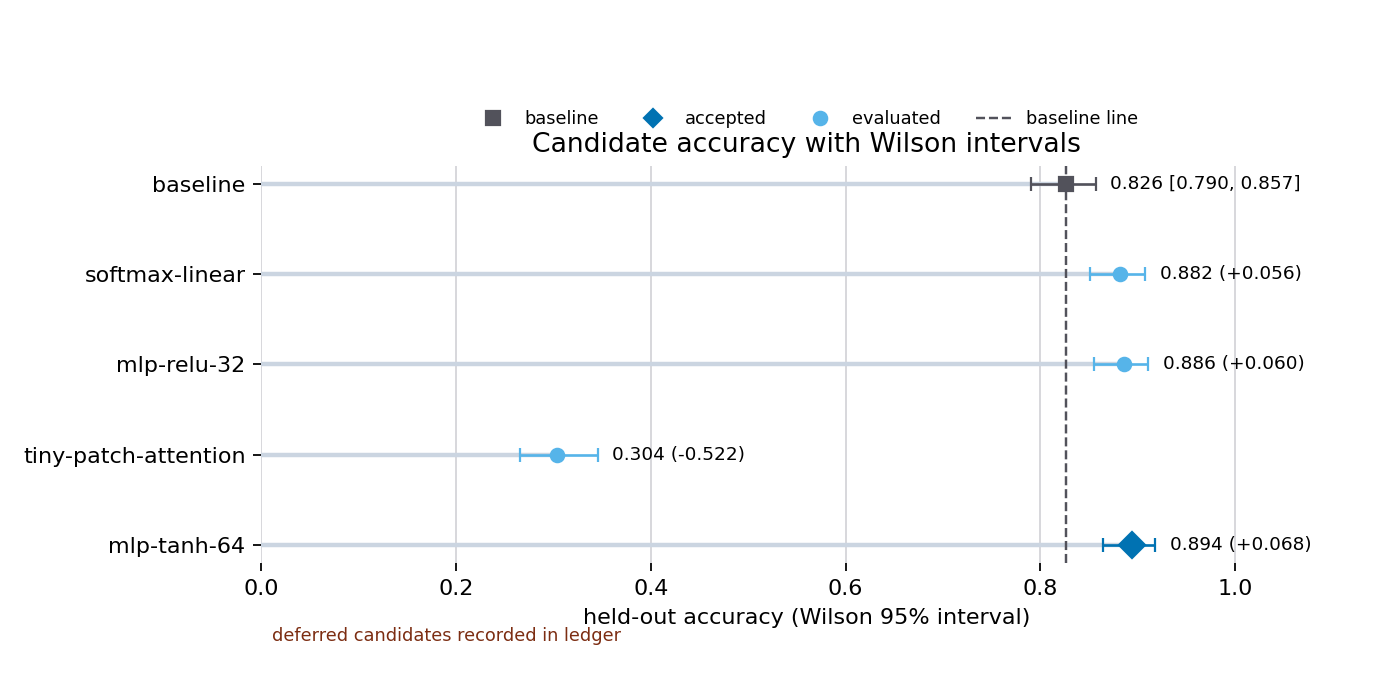
\includegraphics[keepaspectratio,alt={Held-out accuracy with Wilson intervals for the baseline and evaluated candidates from output/data/ml\_candidate\_intervals.json; accepted candidate exp-mlp-tanh-64 improves accuracy from 82.6\% to 89.4\% on the fixed subset, with deferred proposals kept in the candidate ledger. Generation method: Lollipop accuracy comparison with Wilson interval error bars and direct labels. Registry metadata records the generation method, source artifact, and claim boundary for validation.}]{../figures/ml_candidate_scores.png}}
\caption{Held-out accuracy with Wilson intervals for the baseline and
evaluated candidates from output/data/ml\_candidate\_intervals.json;
accepted candidate exp-mlp-tanh-64 improves accuracy from 82.6\% to
89.4\% on the fixed subset, with deferred proposals kept in the
candidate ledger. Generation method: Lollipop accuracy comparison with
Wilson interval error bars and direct labels. Registry metadata records
the generation method, source artifact, and claim boundary for
validation.}\label{fig:ml_candidate_scores}
\end{figure}

\begin{figure}
\centering
\pandocbounded{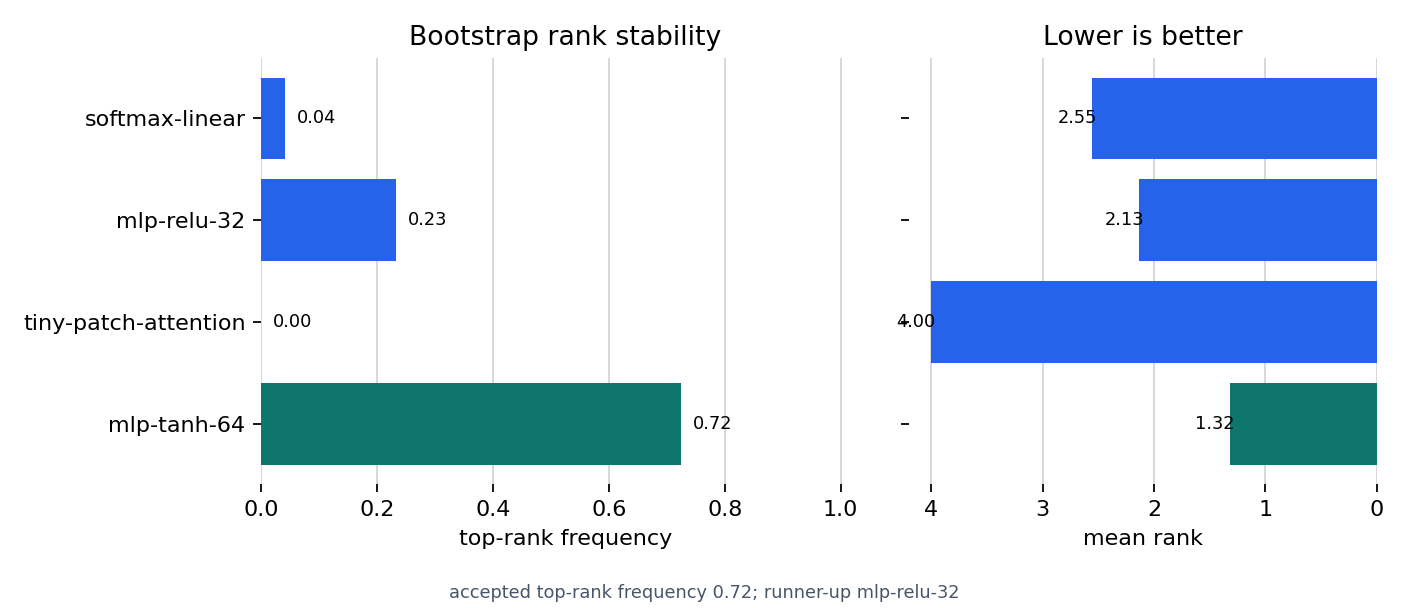
\includegraphics[keepaspectratio,alt={Rank-stability summary for exp-mlp-tanh-64 from output/data/ml\_candidate\_rank\_stability.json; deterministic local bootstrap resampling shows how often each evaluated candidate ranks first under the fixed test split. Generation method: Bootstrap top-rank frequency and mean-rank comparison. Registry metadata records the generation method, source artifact, and claim boundary for validation.}]{../figures/ml_candidate_rank_stability.png}}
\caption{Rank-stability summary for exp-mlp-tanh-64 from
output/data/ml\_candidate\_rank\_stability.json; deterministic local
bootstrap resampling shows how often each evaluated candidate ranks
first under the fixed test split. Generation method: Bootstrap top-rank
frequency and mean-rank comparison. Registry metadata records the
generation method, source artifact, and claim boundary for
validation.}\label{fig:ml_candidate_rank_stability}
\end{figure}

\begin{figure}
\centering
\pandocbounded{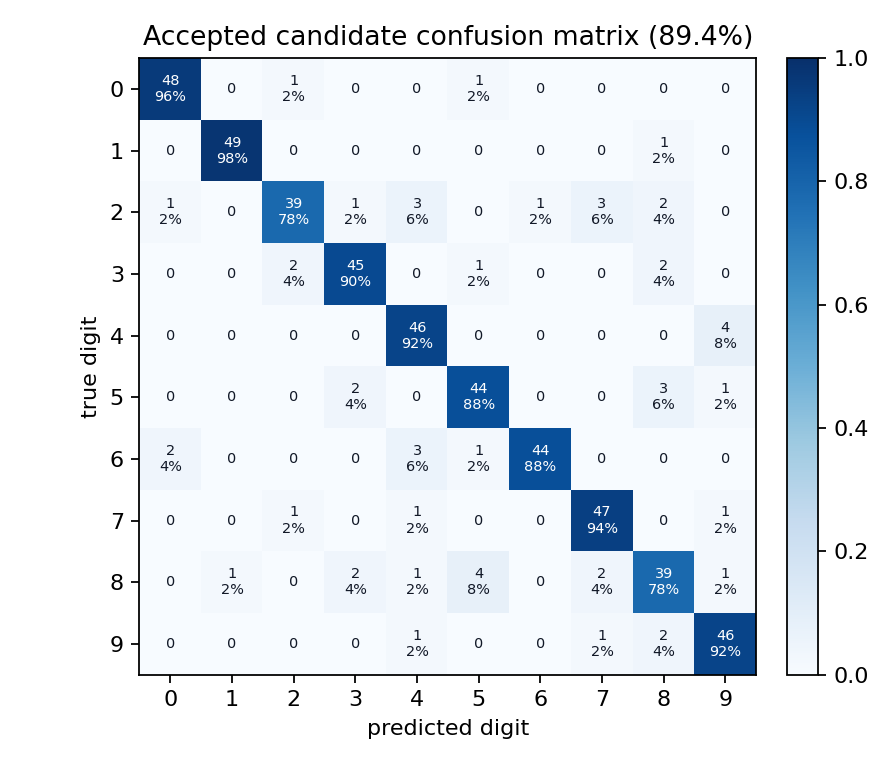
\includegraphics[keepaspectratio,alt={Accepted-candidate confusion matrix for exp-mlp-tanh-64 on the fixed MNIST handwritten digit database test split, sourced from output/data/ml\_confusion\_matrix.csv; it diagnoses the selected run, not general full-dataset performance. Generation method: Row-normalized heatmap with cell counts and row percentages. Registry metadata records the generation method, source artifact, and claim boundary for validation.}]{../figures/ml_confusion_matrix.png}}
\caption{Accepted-candidate confusion matrix for exp-mlp-tanh-64 on the
fixed MNIST handwritten digit database test split, sourced from
output/data/ml\_confusion\_matrix.csv; it diagnoses the selected run,
not general full-dataset performance. Generation method: Row-normalized
heatmap with cell counts and row percentages. Registry metadata records
the generation method, source artifact, and claim boundary for
validation.}\label{fig:ml_confusion_matrix}
\end{figure}

\begin{figure}
\centering
\pandocbounded{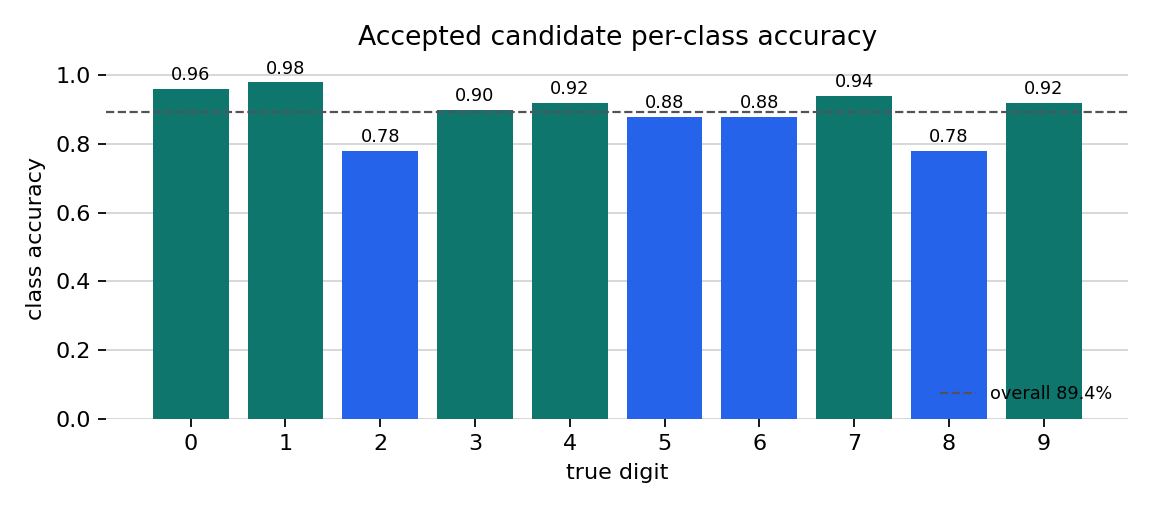
\includegraphics[keepaspectratio,alt={Per-class accuracy for exp-mlp-tanh-64, computed from output/data/ml\_confusion\_matrix.csv; variation across digits is a run diagnostic for the fixed local test split. Generation method: Per-class accuracy bars computed from the confusion matrix diagonal. Registry metadata records the generation method, source artifact, and claim boundary for validation.}]{../figures/ml_per_class_accuracy.png}}
\caption{Per-class accuracy for exp-mlp-tanh-64, computed from
output/data/ml\_confusion\_matrix.csv; variation across digits is a run
diagnostic for the fixed local test split. Generation method: Per-class
accuracy bars computed from the confusion matrix diagonal. Registry
metadata records the generation method, source artifact, and claim
boundary for validation.}\label{fig:ml_per_class_accuracy}
\end{figure}

\subsection{Training And Error
Diagnostics}\label{sec:training-error-diagnostics}

\begin{figure}
\centering
\pandocbounded{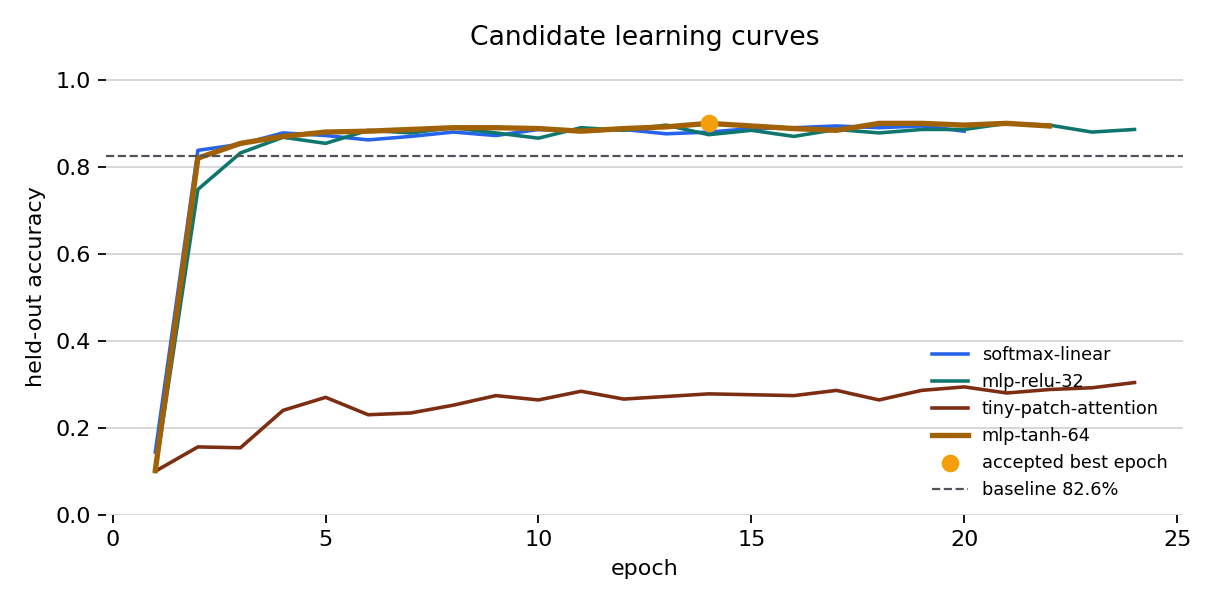
\includegraphics[keepaspectratio,alt={Epoch-level held-out accuracy curves for evaluated candidates from output/data/ml\_training\_history.csv; the accepted curve is visually emphasized for exp-mlp-tanh-64. Generation method: Epoch-level held-out accuracy lines with accepted best-epoch marker. Registry metadata records the generation method, source artifact, and claim boundary for validation.}]{../figures/ml_learning_curves.png}}
\caption{Epoch-level held-out accuracy curves for evaluated candidates
from output/data/ml\_training\_history.csv; the accepted curve is
visually emphasized for exp-mlp-tanh-64. Generation method: Epoch-level
held-out accuracy lines with accepted best-epoch marker. Registry
metadata records the generation method, source artifact, and claim
boundary for validation.}\label{fig:ml_learning_curves}
\end{figure}

\begin{figure}
\centering
\pandocbounded{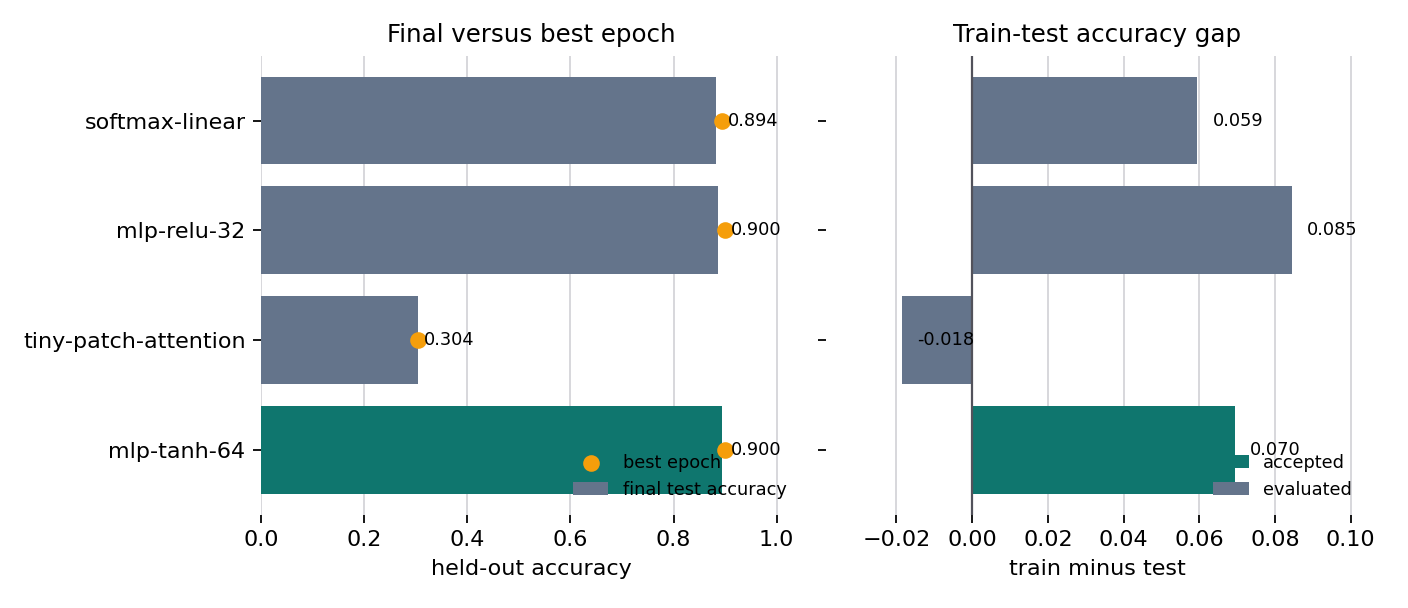
\includegraphics[keepaspectratio,alt={Configured-training dynamics for evaluated candidates from output/data/ml\_training\_diagnostics.json; exp-mlp-tanh-64 is highlighted while best-epoch markers and train-test gaps remain bounded to the local run. Generation method: Final and best-epoch accuracy bars plus train-test gap bars. Registry metadata records the generation method, source artifact, and claim boundary for validation.}]{../figures/ml_training_dynamics.png}}
\caption{Configured-training dynamics for evaluated candidates from
output/data/ml\_training\_diagnostics.json; exp-mlp-tanh-64 is
highlighted while best-epoch markers and train-test gaps remain bounded
to the local run. Generation method: Final and best-epoch accuracy bars
plus train-test gap bars. Registry metadata records the generation
method, source artifact, and claim boundary for
validation.}\label{fig:ml_training_dynamics}
\end{figure}

\begin{figure}
\centering
\pandocbounded{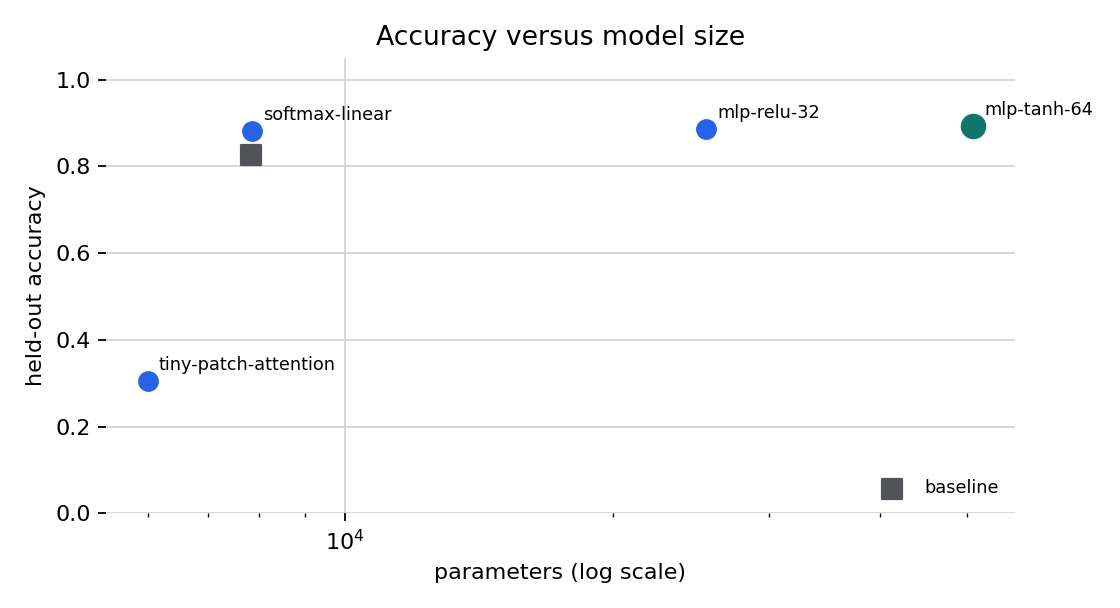
\includegraphics[keepaspectratio,alt={Parameter-count versus held-out accuracy for the baseline and evaluated candidates from output/data/ml\_task\_results.json; the accepted candidate is highlighted without claiming a general scaling law. Generation method: Log-parameter scatter plot against held-out accuracy. Registry metadata records the generation method, source artifact, and claim boundary for validation.}]{../figures/ml_complexity_accuracy.png}}
\caption{Parameter-count versus held-out accuracy for the baseline and
evaluated candidates from output/data/ml\_task\_results.json; the
accepted candidate is highlighted without claiming a general scaling
law. Generation method: Log-parameter scatter plot against held-out
accuracy. Registry metadata records the generation method, source
artifact, and claim boundary for
validation.}\label{fig:ml_complexity_accuracy}
\end{figure}

\begin{figure}
\centering
\pandocbounded{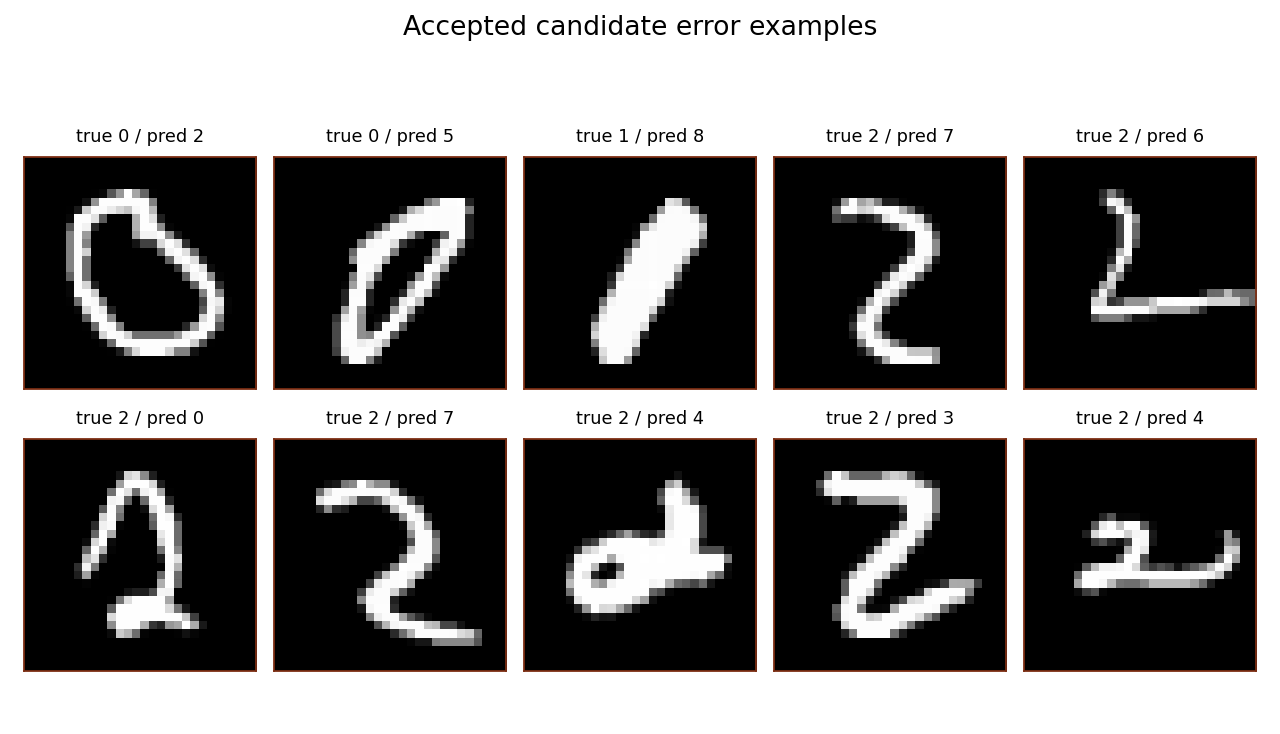
\includegraphics[keepaspectratio,alt={First accepted-candidate error examples for exp-mlp-tanh-64, sourced from output/data/ml\_error\_examples.json and data/mnist\_small.npz; these images support qualitative diagnosis only. Generation method: Deterministic grid of the first accepted-candidate misclassifications. Registry metadata records the generation method, source artifact, and claim boundary for validation.}]{../figures/mnist_error_examples.png}}
\caption{First accepted-candidate error examples for exp-mlp-tanh-64,
sourced from output/data/ml\_error\_examples.json and
data/mnist\_small.npz; these images support qualitative diagnosis only.
Generation method: Deterministic grid of the first accepted-candidate
misclassifications. Registry metadata records the generation method,
source artifact, and claim boundary for
validation.}\label{fig:mnist_error_examples}
\end{figure}

\begin{figure}
\centering
\pandocbounded{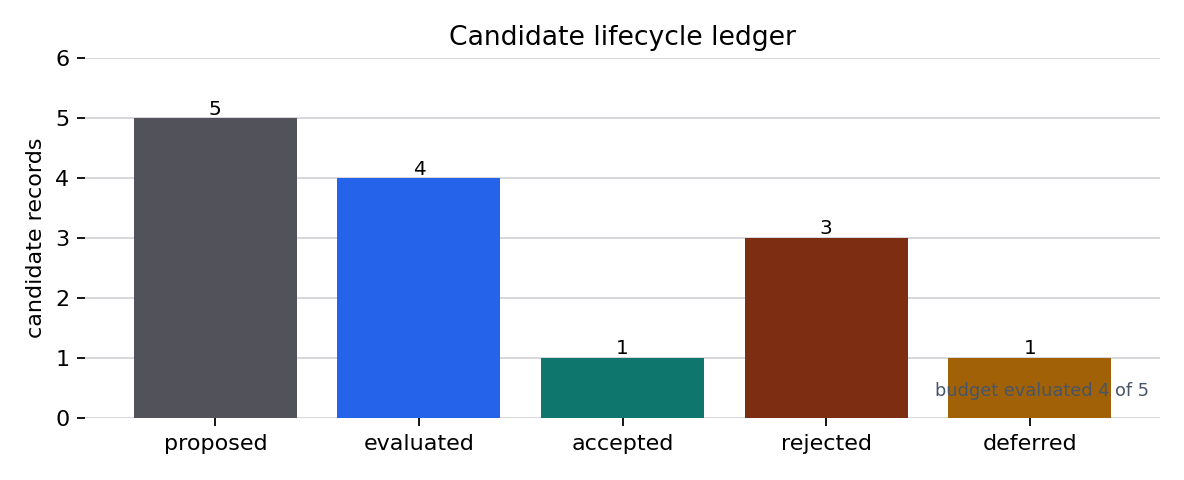
\includegraphics[keepaspectratio,alt={Candidate lifecycle ledger from output/data/ml\_candidate\_ledger.json: 4 evaluated out of 5 proposed candidates, with deferred proposals kept visible instead of executed automatically. Generation method: Candidate lifecycle status-count bar chart. Registry metadata records the generation method, source artifact, and claim boundary for validation.}]{../figures/autoresearch_candidate_lifecycle.png}}
\caption{Candidate lifecycle ledger from
output/data/ml\_candidate\_ledger.json: 4 evaluated out of 5 proposed
candidates, with deferred proposals kept visible instead of executed
automatically. Generation method: Candidate lifecycle status-count bar
chart. Registry metadata records the generation method, source artifact,
and claim boundary for
validation.}\label{fig:autoresearch_candidate_lifecycle}
\end{figure}

The selected candidate's best held-out epoch is \texttt{14}, its final
learning rate is \texttt{0.144}, its train-loss reduction is
\texttt{4.161}, and its final train-test accuracy gap is \texttt{7.0\%}.
These values come from the configured training diagnostics rather than
from a manually maintained result summary.

\begin{longtable}[]{@{}
  >{\raggedright\arraybackslash}p{(\linewidth - 14\tabcolsep) * \real{0.1250}}
  >{\raggedright\arraybackslash}p{(\linewidth - 14\tabcolsep) * \real{0.1250}}
  >{\raggedright\arraybackslash}p{(\linewidth - 14\tabcolsep) * \real{0.1250}}
  >{\raggedright\arraybackslash}p{(\linewidth - 14\tabcolsep) * \real{0.1250}}
  >{\raggedright\arraybackslash}p{(\linewidth - 14\tabcolsep) * \real{0.1250}}
  >{\raggedright\arraybackslash}p{(\linewidth - 14\tabcolsep) * \real{0.1250}}
  >{\raggedright\arraybackslash}p{(\linewidth - 14\tabcolsep) * \real{0.1250}}
  >{\raggedright\arraybackslash}p{(\linewidth - 14\tabcolsep) * \real{0.1250}}@{}}
\caption{Configured-training diagnostics from
\protect\breaktt{output/data/ml\_training\_diagnostics.json}.}\label{tbl:training-diagnostics}\tabularnewline
\toprule\noalign{}
\begin{minipage}[b]{\linewidth}\raggedright
Candidate
\end{minipage} & \begin{minipage}[b]{\linewidth}\raggedright
Status
\end{minipage} & \begin{minipage}[b]{\linewidth}\raggedright
Best epoch
\end{minipage} & \begin{minipage}[b]{\linewidth}\raggedright
Best test accuracy
\end{minipage} & \begin{minipage}[b]{\linewidth}\raggedright
Final test accuracy
\end{minipage} & \begin{minipage}[b]{\linewidth}\raggedright
Train-test gap
\end{minipage} & \begin{minipage}[b]{\linewidth}\raggedright
Loss reduction
\end{minipage} & \begin{minipage}[b]{\linewidth}\raggedright
Final learning rate
\end{minipage} \\
\midrule\noalign{}
\endfirsthead
\toprule\noalign{}
\begin{minipage}[b]{\linewidth}\raggedright
Candidate
\end{minipage} & \begin{minipage}[b]{\linewidth}\raggedright
Status
\end{minipage} & \begin{minipage}[b]{\linewidth}\raggedright
Best epoch
\end{minipage} & \begin{minipage}[b]{\linewidth}\raggedright
Best test accuracy
\end{minipage} & \begin{minipage}[b]{\linewidth}\raggedright
Final test accuracy
\end{minipage} & \begin{minipage}[b]{\linewidth}\raggedright
Train-test gap
\end{minipage} & \begin{minipage}[b]{\linewidth}\raggedright
Loss reduction
\end{minipage} & \begin{minipage}[b]{\linewidth}\raggedright
Final learning rate
\end{minipage} \\
\midrule\noalign{}
\endhead
\bottomrule\noalign{}
\endlastfoot
softmax linear & rejected & 17 & 89.4\% & 88.2\% & 5.9\% & 2.917 &
0.273 \\
mlp relu 32 & rejected & 21 & 90.0\% & 88.6\% & 8.5\% & 4.341 & 0.178 \\
tiny patch attention & rejected & 24 & 30.4\% & 30.4\% & -1.8\% & 0.165
& 0.214 \\
mlp tanh 64 & accepted & 14 & 90.0\% & 89.4\% & 7.0\% & 4.161 & 0.144 \\
\end{longtable}

\subsection{Diagnostic Analysis}\label{sec:diagnostic-analysis}

The selected candidate macro F1 is \texttt{89.4\%}, with a held-out
accuracy interval of \breaktt{86.4\%\ to\ 91.8\%}. Probability
diagnostics report expected calibration error \texttt{2.9\%} and
\texttt{11} high-confidence error(s). The top non-diagonal confusion
pair is \texttt{4\ -\textgreater{}\ 9\ (4)}, and the minimum
selected-candidate accuracy across deterministic robustness transforms
is \texttt{80.0\%}. These values are descriptive diagnostics for the
validated local run, not external benchmark claims.

\subsubsection{Classification And Error
Structure}\label{sec:classification-error-structure}

The class-level and error-pattern diagnostics are intentionally
visual-first: fig.~\ref{fig:ml_calibration_reliability} checks
confidence calibration, fig.~\ref{fig:ml_classification_metrics_heatmap}
separates precision, recall, and F1 by digit, and
fig.~\ref{fig:ml_confusion_pairs} ranks the non-diagonal confusions that
most shape the selected-candidate error profile. The accompanying tables
preserve the same values for audit and downstream comparison.

\begin{figure}
\centering
\pandocbounded{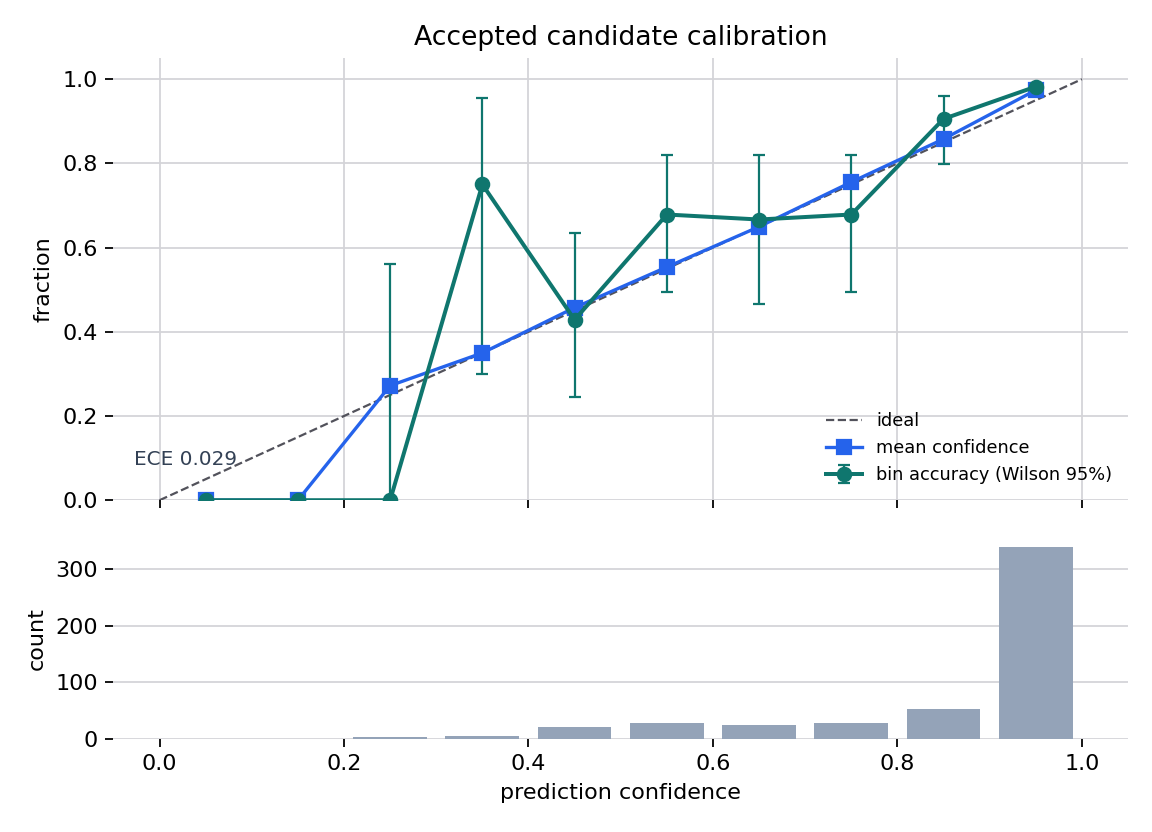
\includegraphics[keepaspectratio,alt={Reliability curve for exp-mlp-tanh-64 from output/data/ml\_calibration\_report.json; expected calibration error and bin counts summarize the accepted candidate on the fixed local test split. Generation method: Reliability curve with confidence-bin support histogram. Registry metadata records the generation method, source artifact, and claim boundary for validation.}]{../figures/ml_calibration_reliability.png}}
\caption{Reliability curve for exp-mlp-tanh-64 from
output/data/ml\_calibration\_report.json; expected calibration error and
bin counts summarize the accepted candidate on the fixed local test
split. Generation method: Reliability curve with confidence-bin support
histogram. Registry metadata records the generation method, source
artifact, and claim boundary for
validation.}\label{fig:ml_calibration_reliability}
\end{figure}

\begin{figure}
\centering
\pandocbounded{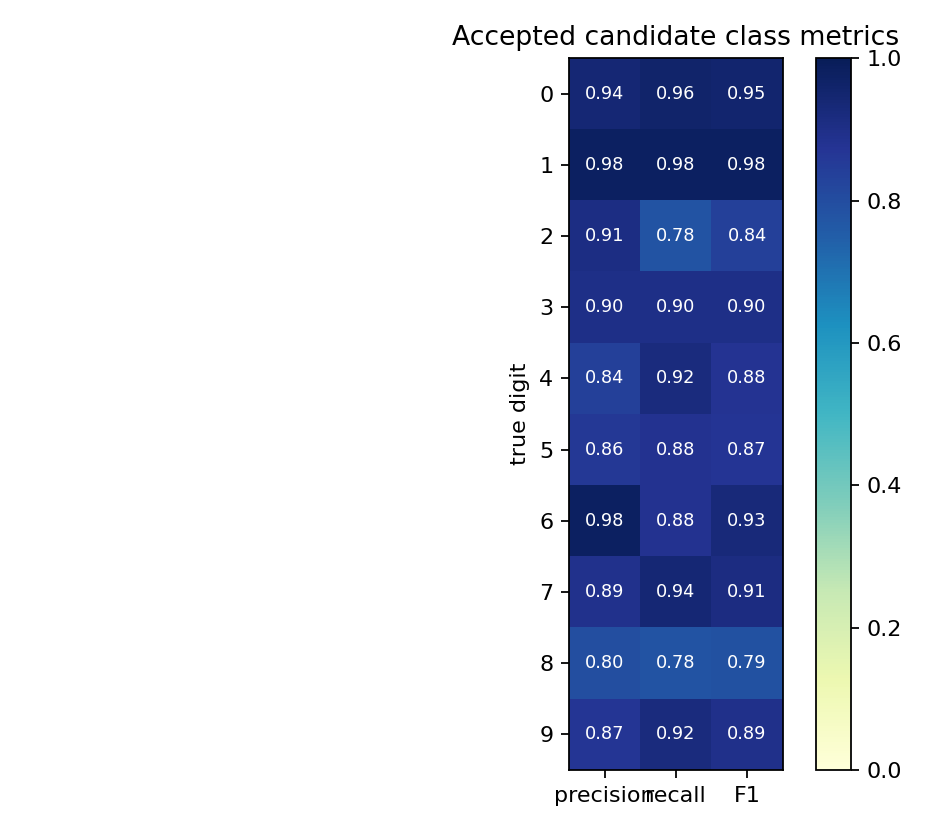
\includegraphics[keepaspectratio,alt={Per-class precision, recall, and F1 for exp-mlp-tanh-64, sourced from output/data/ml\_classification\_diagnostics.json; metrics are scoped to the local test split. Generation method: Per-class precision, recall, and F1 heatmap. Registry metadata records the generation method, source artifact, and claim boundary for validation.}]{../figures/ml_classification_metrics_heatmap.png}}
\caption{Per-class precision, recall, and F1 for exp-mlp-tanh-64,
sourced from output/data/ml\_classification\_diagnostics.json; metrics
are scoped to the local test split. Generation method: Per-class
precision, recall, and F1 heatmap. Registry metadata records the
generation method, source artifact, and claim boundary for
validation.}\label{fig:ml_classification_metrics_heatmap}
\end{figure}

\begin{figure}
\centering
\pandocbounded{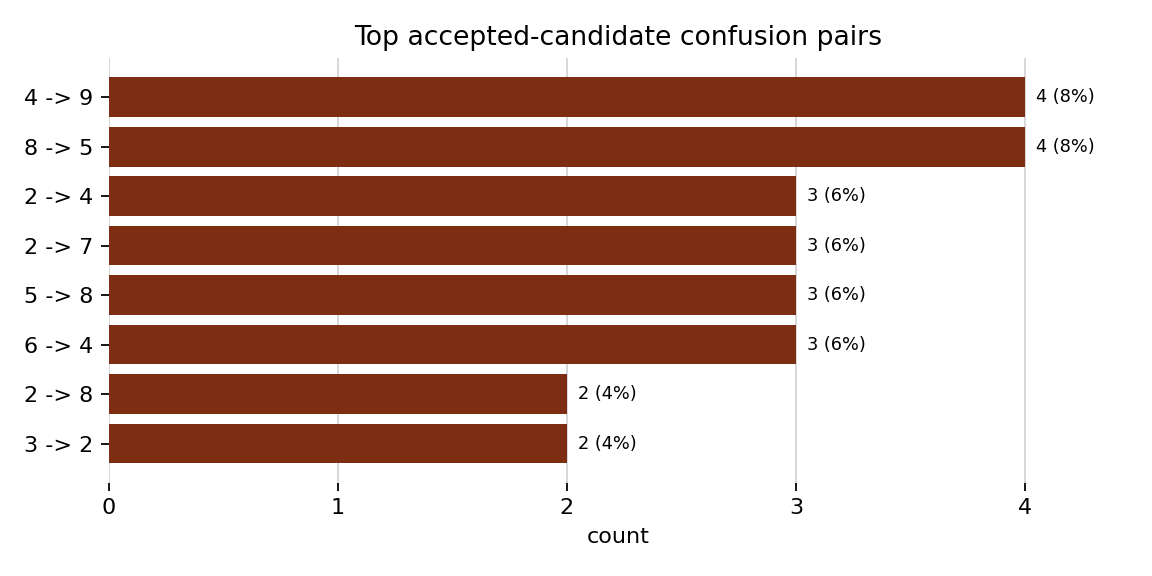
\includegraphics[keepaspectratio,alt={Top non-diagonal confusion pairs for exp-mlp-tanh-64, sourced from output/data/ml\_classification\_diagnostics.json; the bars highlight which local digit pairs account for accepted-candidate errors. Generation method: Ranked off-diagonal confusion-pair bars with true-class error rates. Registry metadata records the generation method, source artifact, and claim boundary for validation.}]{../figures/ml_confusion_pairs.png}}
\caption{Top non-diagonal confusion pairs for exp-mlp-tanh-64, sourced
from output/data/ml\_classification\_diagnostics.json; the bars
highlight which local digit pairs account for accepted-candidate errors.
Generation method: Ranked off-diagonal confusion-pair bars with
true-class error rates. Registry metadata records the generation method,
source artifact, and claim boundary for
validation.}\label{fig:ml_confusion_pairs}
\end{figure}

\begin{longtable}[]{@{}lllll@{}}
\caption{Accepted-candidate class diagnostics from
\protect\breaktt{output/data/ml\_classification\_diagnostics.json}.}\label{tbl:classification-diagnostics}\tabularnewline
\toprule\noalign{}
Class & Precision & Recall & F1 & Support \\
\midrule\noalign{}
\endfirsthead
\toprule\noalign{}
Class & Precision & Recall & F1 & Support \\
\midrule\noalign{}
\endhead
\bottomrule\noalign{}
\endlastfoot
0 & 94.1\% & 96.0\% & 95.0\% & 50 \\
1 & 98.0\% & 98.0\% & 98.0\% & 50 \\
2 & 90.7\% & 78.0\% & 83.9\% & 50 \\
3 & 90.0\% & 90.0\% & 90.0\% & 50 \\
4 & 83.6\% & 92.0\% & 87.6\% & 50 \\
5 & 86.3\% & 88.0\% & 87.1\% & 50 \\
6 & 97.8\% & 88.0\% & 92.6\% & 50 \\
7 & 88.7\% & 94.0\% & 91.3\% & 50 \\
8 & 79.6\% & 78.0\% & 78.8\% & 50 \\
9 & 86.8\% & 92.0\% & 89.3\% & 50 \\
\end{longtable}

\begin{longtable}[]{@{}lllll@{}}
\caption{Calibration bins from
\protect\breaktt{output/data/ml\_calibration\_report.json}.}\label{tbl:calibration-bins}\tabularnewline
\toprule\noalign{}
Confidence bin & Count & Accuracy & Mean confidence & Gap \\
\midrule\noalign{}
\endfirsthead
\toprule\noalign{}
Confidence bin & Count & Accuracy & Mean confidence & Gap \\
\midrule\noalign{}
\endhead
\bottomrule\noalign{}
\endlastfoot
0-0.1 & 0 & 0.0\% & 0.0\% & 0.0\% \\
0.1-0.2 & 0 & 0.0\% & 0.0\% & 0.0\% \\
0.2-0.3 & 3 & 0.0\% & 27.2\% & 27.2\% \\
0.3-0.4 & 4 & 75.0\% & 35.0\% & 40.0\% \\
0.4-0.5 & 21 & 42.9\% & 45.7\% & 2.9\% \\
0.5-0.6 & 28 & 67.9\% & 55.4\% & 12.5\% \\
0.6-0.7 & 24 & 66.7\% & 65.0\% & 1.7\% \\
0.7-0.8 & 28 & 67.9\% & 75.6\% & 7.7\% \\
0.8-0.9 & 53 & 90.6\% & 85.8\% & 4.8\% \\
0.9-1 & 339 & 98.2\% & 97.4\% & 0.8\% \\
\end{longtable}

\begin{longtable}[]{@{}llllll@{}}
\caption{Calibration-bin Wilson intervals from
\protect\breaktt{output/data/ml\_calibration\_bin\_intervals.json}; empty
bins are reported
explicitly.}\label{tbl:calibration-bin-intervals}\tabularnewline
\toprule\noalign{}
Confidence bin & Count & Correct & Accuracy & Wilson 95\% & Empty \\
\midrule\noalign{}
\endfirsthead
\toprule\noalign{}
Confidence bin & Count & Correct & Accuracy & Wilson 95\% & Empty \\
\midrule\noalign{}
\endhead
\bottomrule\noalign{}
\endlastfoot
0-0.1 & 0 & 0 & 0.0\% & 0.0\% to 0.0\% & True \\
0.1-0.2 & 0 & 0 & 0.0\% & 0.0\% to 0.0\% & True \\
0.2-0.3 & 3 & 0 & 0.0\% & 0.0\% to 56.2\% & False \\
0.3-0.4 & 4 & 3 & 75.0\% & 30.1\% to 95.4\% & False \\
0.4-0.5 & 21 & 9 & 42.9\% & 24.5\% to 63.5\% & False \\
0.5-0.6 & 28 & 19 & 67.9\% & 49.3\% to 82.1\% & False \\
0.6-0.7 & 24 & 16 & 66.7\% & 46.7\% to 82.0\% & False \\
0.7-0.8 & 28 & 19 & 67.9\% & 49.3\% to 82.1\% & False \\
0.8-0.9 & 53 & 48 & 90.6\% & 79.7\% to 95.9\% & False \\
0.9-1 & 339 & 333 & 98.2\% & 96.2\% to 99.2\% & False \\
\end{longtable}

\begin{longtable}[]{@{}lll@{}}
\caption{Top non-diagonal confusion pairs from
\protect\breaktt{output/data/ml\_classification\_diagnostics.json}.}\label{tbl:confusion-pairs}\tabularnewline
\toprule\noalign{}
Pair & Count & True-class error rate \\
\midrule\noalign{}
\endfirsthead
\toprule\noalign{}
Pair & Count & True-class error rate \\
\midrule\noalign{}
\endhead
\bottomrule\noalign{}
\endlastfoot
4 -\textgreater{} 9 & 4 & 8.0\% \\
8 -\textgreater{} 5 & 4 & 8.0\% \\
2 -\textgreater{} 4 & 3 & 6.0\% \\
2 -\textgreater{} 7 & 3 & 6.0\% \\
5 -\textgreater{} 8 & 3 & 6.0\% \\
6 -\textgreater{} 4 & 3 & 6.0\% \\
2 -\textgreater{} 8 & 2 & 4.0\% \\
3 -\textgreater{} 2 & 2 & 4.0\% \\
3 -\textgreater{} 8 & 2 & 4.0\% \\
5 -\textgreater{} 3 & 2 & 4.0\% \\
\end{longtable}

\subsubsection{Uncertainty, Generalization, And
Perturbation}\label{sec:uncertainty-generalization-perturbation}

Additional uncertainty and matched-comparison diagnostics report
bootstrap accuracy interval \breaktt{86.4\%\ to\ 92.0\%}, bootstrap
macro-F1 interval \breaktt{86.5\%\ to\ 91.9\%}, paired net accuracy gain
\texttt{6.8\%}, exact McNemar p-value \texttt{0.000}, mean
correct-prediction confidence \texttt{90.9\%}, mean error confidence
\texttt{63.1\%}, and \texttt{22} low-margin selected-candidate
prediction(s). These diagnostics are generated from the fixed local test
split and are reported as run evidence, not as population-level
certification.

fig.~\ref{fig:ml_generalization_gap} compares train and test behavior,
fig.~\ref{fig:ml_robustness_matrix} shows deterministic no-retrain
perturbation results, fig.~\ref{fig:ml_probability_margin_distribution}
summarizes confidence and margin distributions,
fig.~\ref{fig:ml_bootstrap_intervals} shows local resampling intervals,
and fig.~\ref{fig:ml_paired_correctness} exposes the matched
selected-versus-baseline correctness table used by the paired
comparison.

\begin{figure}
\centering
\pandocbounded{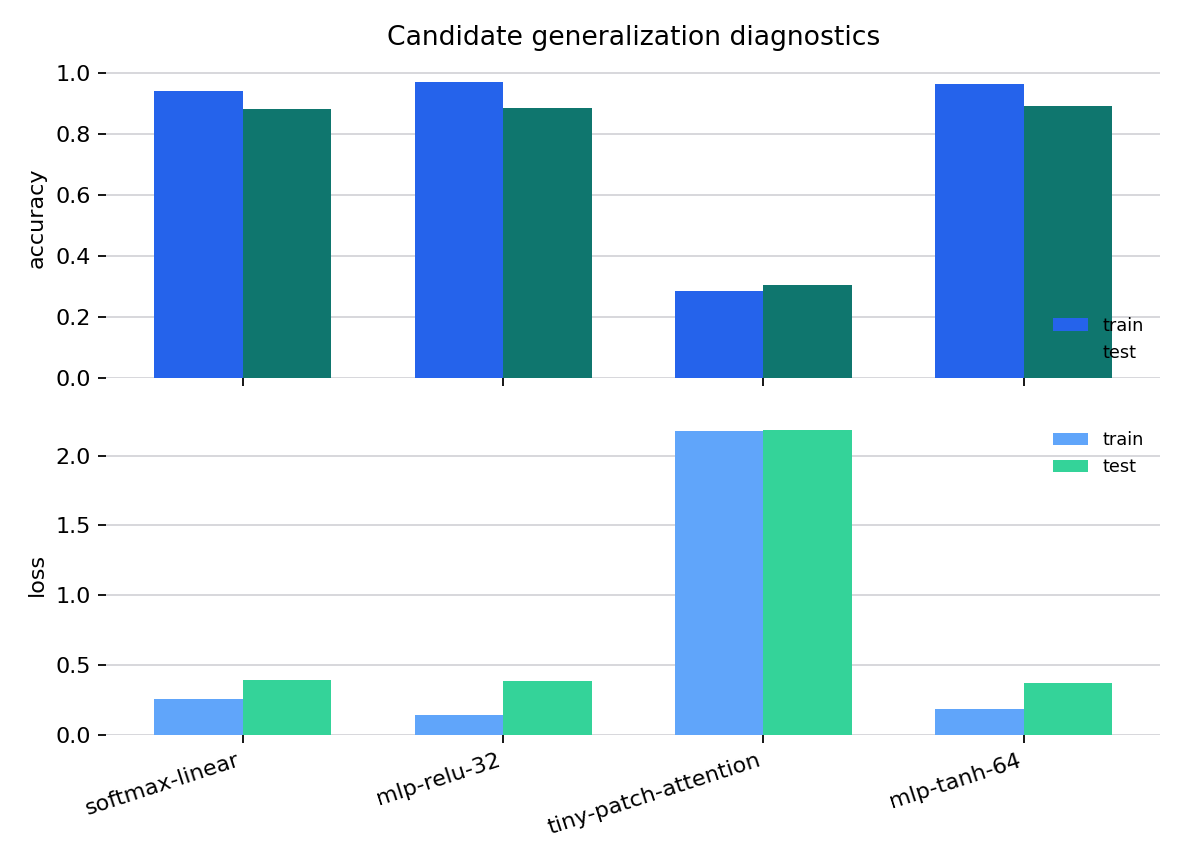
\includegraphics[keepaspectratio,alt={Train/test accuracy and loss for evaluated candidates from output/data/ml\_classification\_diagnostics.json; the plot exposes local generalization gaps without claiming full-dataset behavior. Generation method: Grouped train/test accuracy and loss bars by evaluated candidate. Registry metadata records the generation method, source artifact, and claim boundary for validation.}]{../figures/ml_generalization_gap.png}}
\caption{Train/test accuracy and loss for evaluated candidates from
output/data/ml\_classification\_diagnostics.json; the plot exposes local
generalization gaps without claiming full-dataset behavior. Generation
method: Grouped train/test accuracy and loss bars by evaluated
candidate. Registry metadata records the generation method, source
artifact, and claim boundary for
validation.}\label{fig:ml_generalization_gap}
\end{figure}

\begin{figure}
\centering
\pandocbounded{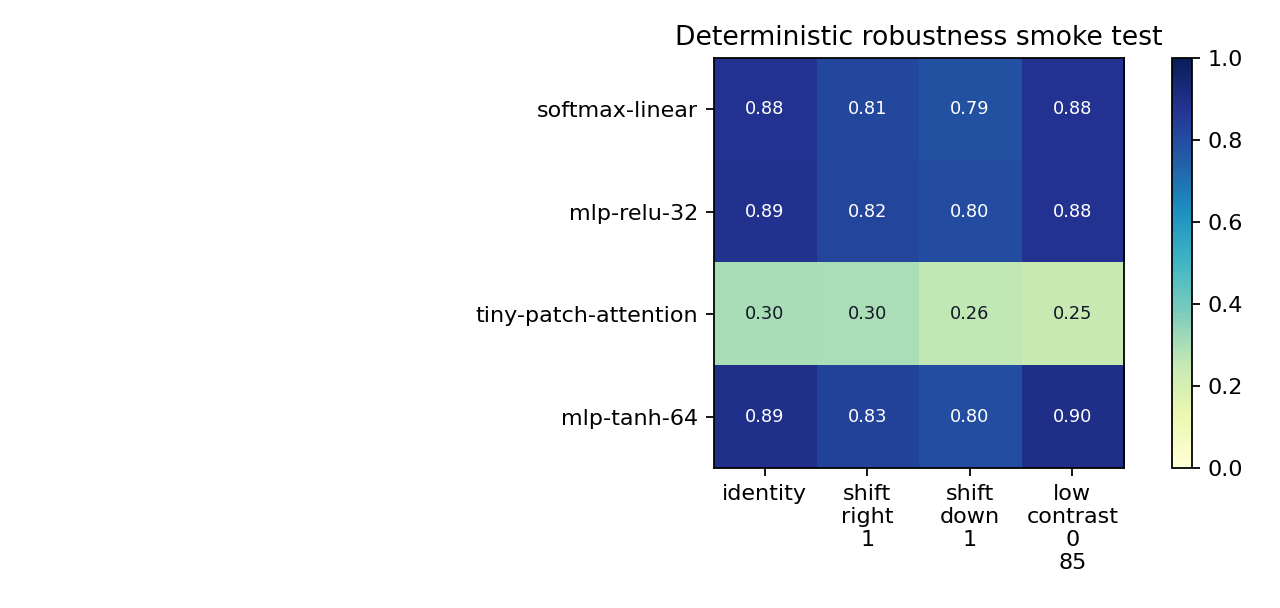
\includegraphics[keepaspectratio,alt={Accuracy for evaluated candidates under identity, one-pixel shifts, and low contrast from output/data/ml\_robustness\_report.json; the deterministic transforms provide a bounded smoke test only. Generation method: Candidate-by-transform accuracy heatmap for deterministic perturbations. Registry metadata records the generation method, source artifact, and claim boundary for validation.}]{../figures/ml_robustness_matrix.png}}
\caption{Accuracy for evaluated candidates under identity, one-pixel
shifts, and low contrast from output/data/ml\_robustness\_report.json;
the deterministic transforms provide a bounded smoke test only.
Generation method: Candidate-by-transform accuracy heatmap for
deterministic perturbations. Registry metadata records the generation
method, source artifact, and claim boundary for
validation.}\label{fig:ml_robustness_matrix}
\end{figure}

\begin{figure}
\centering
\pandocbounded{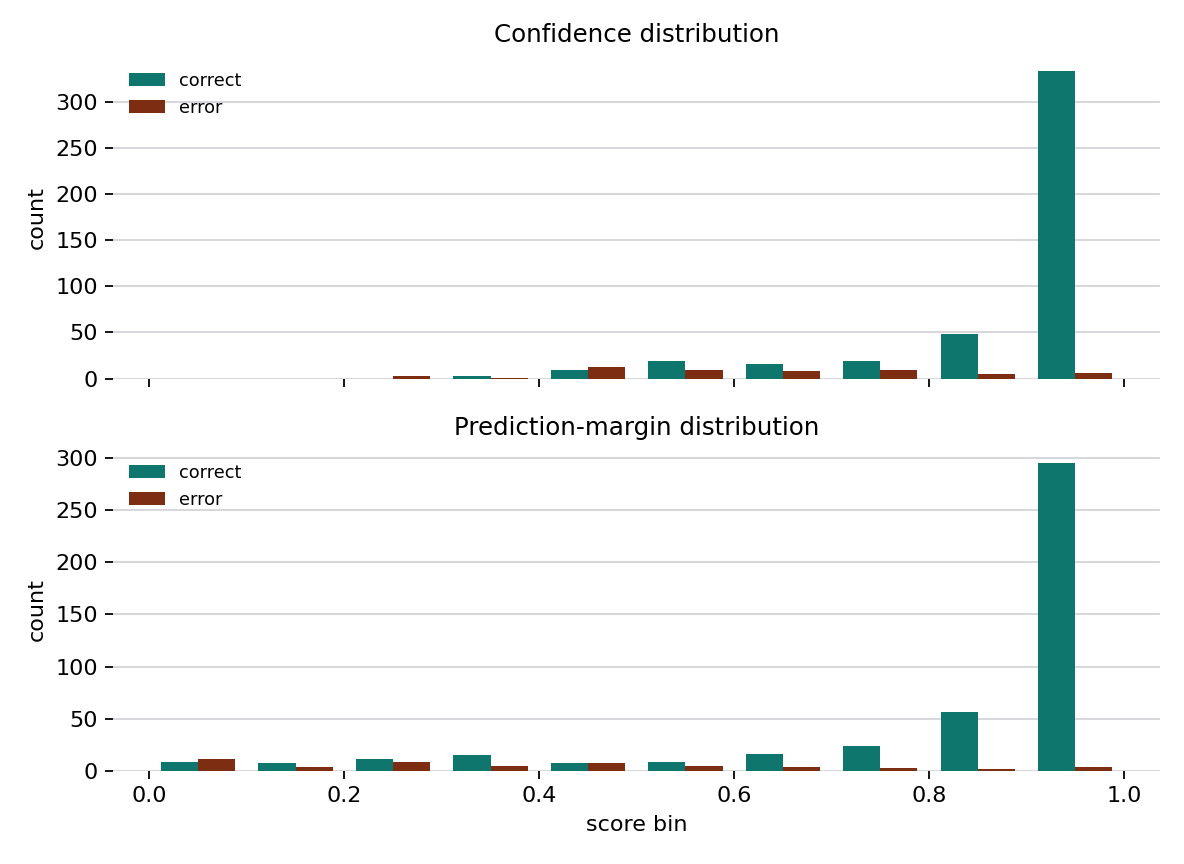
\includegraphics[keepaspectratio,alt={Confidence and prediction-margin histograms for exp-mlp-tanh-64 from output/data/ml\_probability\_diagnostics.json; the figure separates correct and incorrect local test predictions. Generation method: Confidence and margin histograms split by correctness. Registry metadata records the generation method, source artifact, and claim boundary for validation.}]{../figures/ml_probability_margin_distribution.png}}
\caption{Confidence and prediction-margin histograms for exp-mlp-tanh-64
from output/data/ml\_probability\_diagnostics.json; the figure separates
correct and incorrect local test predictions. Generation method:
Confidence and margin histograms split by correctness. Registry metadata
records the generation method, source artifact, and claim boundary for
validation.}\label{fig:ml_probability_margin_distribution}
\end{figure}

\begin{figure}
\centering
\pandocbounded{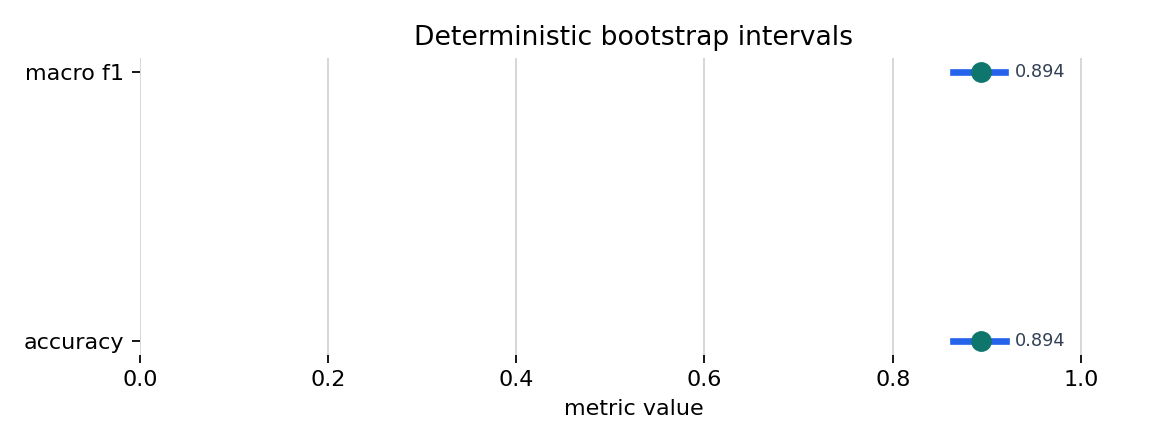
\includegraphics[keepaspectratio,alt={Deterministic percentile-bootstrap intervals for exp-mlp-tanh-64 from output/data/ml\_bootstrap\_intervals.json; the intervals summarize local sampling variation for accuracy and macro F1. Generation method: Horizontal percentile-bootstrap interval plot. Registry metadata records the generation method, source artifact, and claim boundary for validation.}]{../figures/ml_bootstrap_intervals.png}}
\caption{Deterministic percentile-bootstrap intervals for
exp-mlp-tanh-64 from output/data/ml\_bootstrap\_intervals.json; the
intervals summarize local sampling variation for accuracy and macro F1.
Generation method: Horizontal percentile-bootstrap interval plot.
Registry metadata records the generation method, source artifact, and
claim boundary for validation.}\label{fig:ml_bootstrap_intervals}
\end{figure}

\begin{figure}
\centering
\pandocbounded{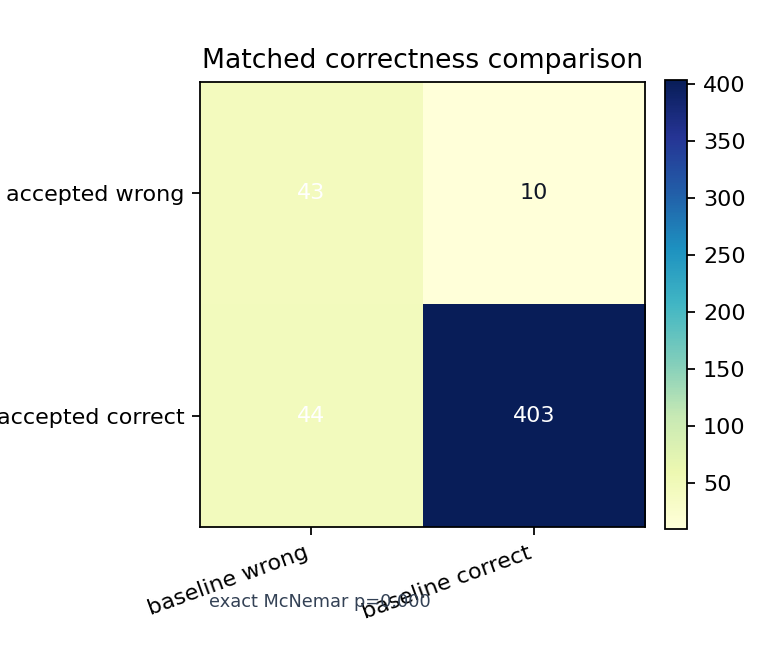
\includegraphics[keepaspectratio,alt={Matched correctness comparison between exp-mlp-tanh-64 and the nearest\_centroid\_baseline baseline from output/data/ml\_paired\_comparison.json; discordant cells support the paired test summary. Generation method: Matched accepted-versus-baseline correctness heatmap. Registry metadata records the generation method, source artifact, and claim boundary for validation.}]{../figures/ml_paired_correctness.png}}
\caption{Matched correctness comparison between exp-mlp-tanh-64 and the
nearest\_centroid\_baseline baseline from
output/data/ml\_paired\_comparison.json; discordant cells support the
paired test summary. Generation method: Matched accepted-versus-baseline
correctness heatmap. Registry metadata records the generation method,
source artifact, and claim boundary for
validation.}\label{fig:ml_paired_correctness}
\end{figure}

\begin{longtable}[]{@{}llll@{}}
\caption{Deterministic no-retrain robustness smoke test from
\protect\breaktt{output/data/ml\_robustness\_report.json}.}\label{tbl:robustness-scores}\tabularnewline
\toprule\noalign{}
Candidate & Transform & Accuracy & Samples \\
\midrule\noalign{}
\endfirsthead
\toprule\noalign{}
Candidate & Transform & Accuracy & Samples \\
\midrule\noalign{}
\endhead
\bottomrule\noalign{}
\endlastfoot
softmax linear & identity & 88.2\% & 500 \\
softmax linear & shift\_right\_1 & 81.4\% & 500 \\
softmax linear & shift\_down\_1 & 78.6\% & 500 \\
softmax linear & low\_contrast\_0\_85 & 88.0\% & 500 \\
mlp relu 32 & identity & 88.6\% & 500 \\
mlp relu 32 & shift\_right\_1 & 82.4\% & 500 \\
mlp relu 32 & shift\_down\_1 & 80.2\% & 500 \\
mlp relu 32 & low\_contrast\_0\_85 & 88.2\% & 500 \\
tiny patch attention & identity & 30.4\% & 500 \\
tiny patch attention & shift\_right\_1 & 29.8\% & 500 \\
tiny patch attention & shift\_down\_1 & 25.8\% & 500 \\
tiny patch attention & low\_contrast\_0\_85 & 24.6\% & 500 \\
mlp tanh 64 & identity & 89.4\% & 500 \\
mlp tanh 64 & shift\_right\_1 & 83.2\% & 500 \\
mlp tanh 64 & shift\_down\_1 & 80.0\% & 500 \\
mlp tanh 64 & low\_contrast\_0\_85 & 89.8\% & 500 \\
\end{longtable}

\begin{longtable}[]{@{}ll@{}}
\caption{Accepted-candidate probability diagnostics from
\protect\breaktt{output/data/ml\_probability\_diagnostics.json}.}\label{tbl:probability-diagnostics}\tabularnewline
\toprule\noalign{}
Statistic & Value \\
\midrule\noalign{}
\endfirsthead
\toprule\noalign{}
Statistic & Value \\
\midrule\noalign{}
\endhead
\bottomrule\noalign{}
\endlastfoot
Mean confidence & 87.9\% \\
Mean correct confidence & 90.9\% \\
Mean error confidence & 63.1\% \\
Mean margin & 80.2\% \\
Mean correct margin & 84.9\% \\
Mean error margin & 40.3\% \\
Low-margin count & 22 \\
\end{longtable}

\begin{longtable}[]{@{}lllll@{}}
\caption{Deterministic percentile-bootstrap intervals from
\protect\breaktt{output/data/ml\_bootstrap\_intervals.json}.}\label{tbl:bootstrap-intervals}\tabularnewline
\toprule\noalign{}
Metric & Observed & CI low & CI high & Resample mean \\
\midrule\noalign{}
\endfirsthead
\toprule\noalign{}
Metric & Observed & CI low & CI high & Resample mean \\
\midrule\noalign{}
\endhead
\bottomrule\noalign{}
\endlastfoot
accuracy & 89.4\% & 86.4\% & 92.0\% & 89.4\% \\
macro F1 & 89.4\% & 86.5\% & 91.9\% & 89.3\% \\
\end{longtable}

\begin{longtable}[]{@{}ll@{}}
\caption{Accepted-candidate versus baseline paired comparison from
\protect\breaktt{output/data/ml\_paired\_comparison.json}.}\label{tbl:paired-comparison}\tabularnewline
\toprule\noalign{}
Matched comparison statistic & Value \\
\midrule\noalign{}
\endfirsthead
\toprule\noalign{}
Matched comparison statistic & Value \\
\midrule\noalign{}
\endhead
\bottomrule\noalign{}
\endlastfoot
Both correct & 403 \\
Accepted only correct & 44 \\
Baseline only correct & 10 \\
Both wrong & 43 \\
Discordant examples & 54 \\
Exact McNemar p & 0.000 \\
Net accuracy gain & 6.8\% \\
\end{longtable}

\subsubsection{Probability Quality And Selective
Prediction}\label{sec:probability-quality-selective-prediction}

Probability-quality diagnostics report Brier score \texttt{0.161},
negative log likelihood \texttt{0.361}, top-2 accuracy \texttt{95.6\%},
and Cohen kappa \texttt{0.882} for the selected candidate. At the
highest configured confidence threshold, retained coverage is
\texttt{67.8\%} and selective accuracy is \texttt{98.2\%}.

The selective-prediction view in fig.~\ref{fig:ml_selective_accuracy}
reports the configured confidence-threshold trade-off: retaining fewer
predictions can raise selective accuracy, but the coverage table keeps
that trade-off explicit. The candidate probability-quality comparison in
fig.~\ref{fig:ml_probability_quality} keeps accuracy separate from
proper-score behavior, so the selected candidate is not treated as
automatically best on every diagnostic axis.

\begin{figure}
\centering
\pandocbounded{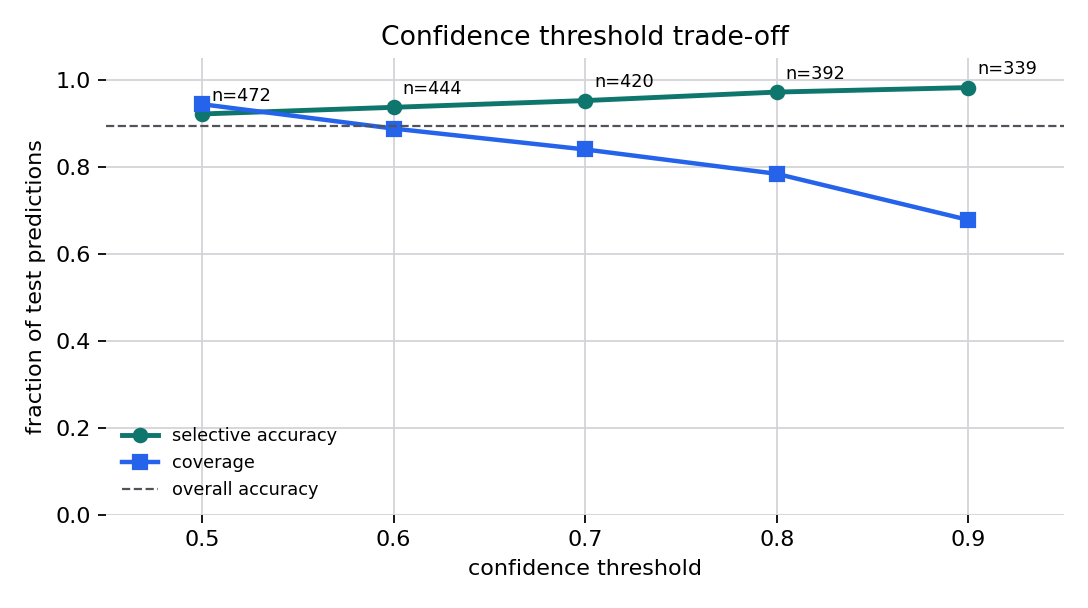
\includegraphics[keepaspectratio,alt={Confidence-threshold trade-off for exp-mlp-tanh-64 from output/data/ml\_statistical\_summary.json; the plot compares retained coverage, selective accuracy, and the unthresholded accepted-candidate accuracy on the fixed local split. Generation method: Confidence-threshold coverage and selective-accuracy line chart. Registry metadata records the generation method, source artifact, and claim boundary for validation.}]{../figures/ml_selective_accuracy.png}}
\caption{Confidence-threshold trade-off for exp-mlp-tanh-64 from
output/data/ml\_statistical\_summary.json; the plot compares retained
coverage, selective accuracy, and the unthresholded accepted-candidate
accuracy on the fixed local split. Generation method:
Confidence-threshold coverage and selective-accuracy line chart.
Registry metadata records the generation method, source artifact, and
claim boundary for validation.}\label{fig:ml_selective_accuracy}
\end{figure}

\begin{figure}
\centering
\pandocbounded{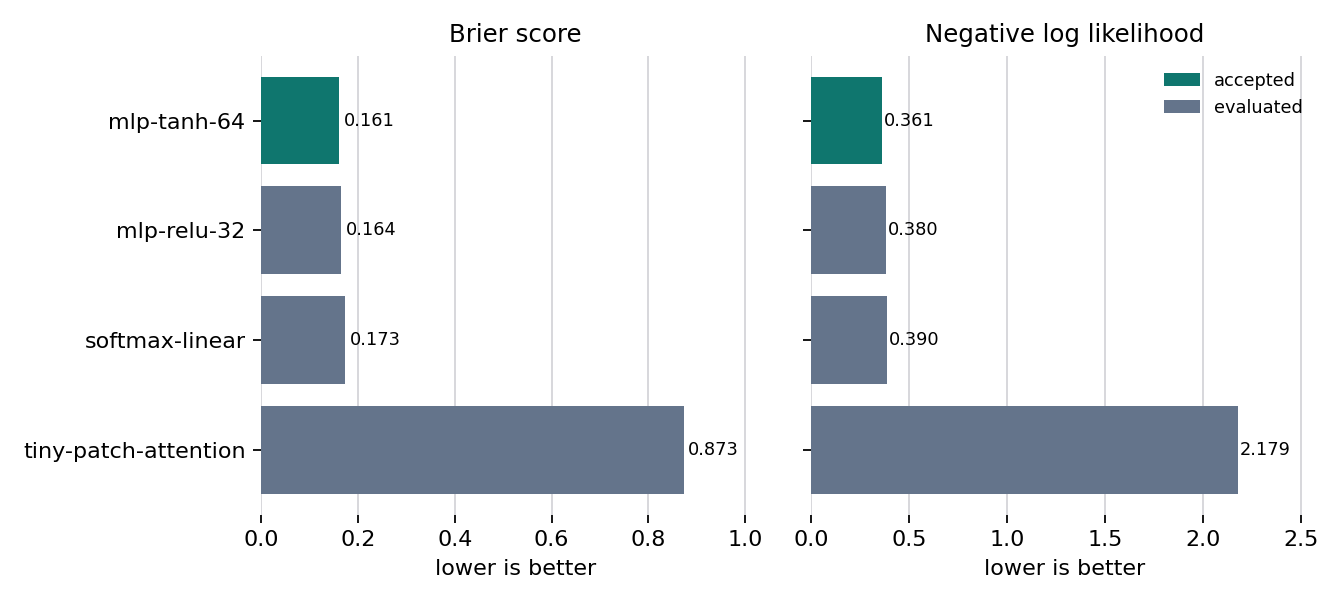
\includegraphics[keepaspectratio,alt={Brier score and negative log likelihood for evaluated candidates from output/data/ml\_statistical\_summary.json; lower values indicate better probability quality within the configured local run, and the accepted candidate is highlighted. Generation method: Brier score and negative-log-likelihood bar comparison. Registry metadata records the generation method, source artifact, and claim boundary for validation.}]{../figures/ml_probability_quality.png}}
\caption{Brier score and negative log likelihood for evaluated
candidates from output/data/ml\_statistical\_summary.json; lower values
indicate better probability quality within the configured local run, and
the accepted candidate is highlighted. Generation method: Brier score
and negative-log-likelihood bar comparison. Registry metadata records
the generation method, source artifact, and claim boundary for
validation.}\label{fig:ml_probability_quality}
\end{figure}

\begin{longtable}[]{@{}ll@{}}
\caption{Accepted-candidate statistical summary from
\protect\breaktt{output/data/ml\_statistical\_summary.json}.}\label{tbl:statistical-summary}\tabularnewline
\toprule\noalign{}
Statistic & Value \\
\midrule\noalign{}
\endfirsthead
\toprule\noalign{}
Statistic & Value \\
\midrule\noalign{}
\endhead
\bottomrule\noalign{}
\endlastfoot
Accuracy & 89.4\% \\
Balanced accuracy & 89.4\% \\
Macro F1 & 89.4\% \\
Top-2 accuracy & 95.6\% \\
Cohen kappa & 0.882 \\
Brier score & 0.161 \\
Negative log likelihood & 0.361 \\
Expected calibration error & 2.9\% \\
\end{longtable}

\begin{longtable}[]{@{}
  >{\raggedright\arraybackslash}p{(\linewidth - 8\tabcolsep) * \real{0.2000}}
  >{\raggedright\arraybackslash}p{(\linewidth - 8\tabcolsep) * \real{0.2000}}
  >{\raggedright\arraybackslash}p{(\linewidth - 8\tabcolsep) * \real{0.2000}}
  >{\raggedright\arraybackslash}p{(\linewidth - 8\tabcolsep) * \real{0.2000}}
  >{\raggedright\arraybackslash}p{(\linewidth - 8\tabcolsep) * \real{0.2000}}@{}}
\caption{Selective-accuracy threshold table from
\protect\breaktt{output/data/ml\_statistical\_summary.json}.}\label{tbl:selective-accuracy}\tabularnewline
\toprule\noalign{}
\begin{minipage}[b]{\linewidth}\raggedright
Confidence threshold
\end{minipage} & \begin{minipage}[b]{\linewidth}\raggedright
Coverage
\end{minipage} & \begin{minipage}[b]{\linewidth}\raggedright
Selective accuracy
\end{minipage} & \begin{minipage}[b]{\linewidth}\raggedright
Retained
\end{minipage} & \begin{minipage}[b]{\linewidth}\raggedright
Errors
\end{minipage} \\
\midrule\noalign{}
\endfirsthead
\toprule\noalign{}
\begin{minipage}[b]{\linewidth}\raggedright
Confidence threshold
\end{minipage} & \begin{minipage}[b]{\linewidth}\raggedright
Coverage
\end{minipage} & \begin{minipage}[b]{\linewidth}\raggedright
Selective accuracy
\end{minipage} & \begin{minipage}[b]{\linewidth}\raggedright
Retained
\end{minipage} & \begin{minipage}[b]{\linewidth}\raggedright
Errors
\end{minipage} \\
\midrule\noalign{}
\endhead
\bottomrule\noalign{}
\endlastfoot
50.0\% & 94.4\% & 92.2\% & 472 & 37 \\
60.0\% & 88.8\% & 93.7\% & 444 & 28 \\
70.0\% & 84.0\% & 95.2\% & 420 & 20 \\
80.0\% & 78.4\% & 97.2\% & 392 & 11 \\
90.0\% & 67.8\% & 98.2\% & 339 & 6 \\
\end{longtable}

\begin{longtable}[]{@{}
  >{\raggedright\arraybackslash}p{(\linewidth - 10\tabcolsep) * \real{0.1667}}
  >{\raggedright\arraybackslash}p{(\linewidth - 10\tabcolsep) * \real{0.1667}}
  >{\raggedright\arraybackslash}p{(\linewidth - 10\tabcolsep) * \real{0.1667}}
  >{\raggedright\arraybackslash}p{(\linewidth - 10\tabcolsep) * \real{0.1667}}
  >{\raggedright\arraybackslash}p{(\linewidth - 10\tabcolsep) * \real{0.1667}}
  >{\raggedright\arraybackslash}p{(\linewidth - 10\tabcolsep) * \real{0.1667}}@{}}
\caption{Candidate probability-quality table from
\protect\breaktt{output/data/ml\_statistical\_summary.json}.}\label{tbl:probability-quality}\tabularnewline
\toprule\noalign{}
\begin{minipage}[b]{\linewidth}\raggedright
Candidate
\end{minipage} & \begin{minipage}[b]{\linewidth}\raggedright
Accuracy
\end{minipage} & \begin{minipage}[b]{\linewidth}\raggedright
Top-2 accuracy
\end{minipage} & \begin{minipage}[b]{\linewidth}\raggedright
Brier
\end{minipage} & \begin{minipage}[b]{\linewidth}\raggedright
NLL
\end{minipage} & \begin{minipage}[b]{\linewidth}\raggedright
Mean confidence
\end{minipage} \\
\midrule\noalign{}
\endfirsthead
\toprule\noalign{}
\begin{minipage}[b]{\linewidth}\raggedright
Candidate
\end{minipage} & \begin{minipage}[b]{\linewidth}\raggedright
Accuracy
\end{minipage} & \begin{minipage}[b]{\linewidth}\raggedright
Top-2 accuracy
\end{minipage} & \begin{minipage}[b]{\linewidth}\raggedright
Brier
\end{minipage} & \begin{minipage}[b]{\linewidth}\raggedright
NLL
\end{minipage} & \begin{minipage}[b]{\linewidth}\raggedright
Mean confidence
\end{minipage} \\
\midrule\noalign{}
\endhead
\bottomrule\noalign{}
\endlastfoot
softmax linear & 88.2\% & 95.8\% & 0.173 & 0.390 & 85.1\% \\
mlp relu 32 & 88.6\% & 95.6\% & 0.164 & 0.380 & 89.9\% \\
tiny patch attention & 30.4\% & 46.6\% & 0.873 & 2.179 & 13.1\% \\
mlp tanh 64 & 89.4\% & 95.6\% & 0.161 & 0.361 & 87.9\% \\
\end{longtable}

\subsection{Candidate Ledger}\label{sec:candidate-ledger}

\begin{longtable}[]{@{}
  >{\raggedright\arraybackslash}p{(\linewidth - 8\tabcolsep) * \real{0.2000}}
  >{\raggedright\arraybackslash}p{(\linewidth - 8\tabcolsep) * \real{0.2000}}
  >{\raggedright\arraybackslash}p{(\linewidth - 8\tabcolsep) * \real{0.2000}}
  >{\raggedright\arraybackslash}p{(\linewidth - 8\tabcolsep) * \real{0.2000}}
  >{\raggedright\arraybackslash}p{(\linewidth - 8\tabcolsep) * \real{0.2000}}@{}}
\caption{Candidate lifecycle ledger from
\protect\breaktt{output/data/ml\_candidate\_ledger.json}.}\label{tbl:ml-candidate-ledger}\tabularnewline
\toprule\noalign{}
\begin{minipage}[b]{\linewidth}\raggedright
Candidate
\end{minipage} & \begin{minipage}[b]{\linewidth}\raggedright
Model
\end{minipage} & \begin{minipage}[b]{\linewidth}\raggedright
Status
\end{minipage} & \begin{minipage}[b]{\linewidth}\raggedright
Test accuracy
\end{minipage} & \begin{minipage}[b]{\linewidth}\raggedright
Parameters
\end{minipage} \\
\midrule\noalign{}
\endfirsthead
\toprule\noalign{}
\begin{minipage}[b]{\linewidth}\raggedright
Candidate
\end{minipage} & \begin{minipage}[b]{\linewidth}\raggedright
Model
\end{minipage} & \begin{minipage}[b]{\linewidth}\raggedright
Status
\end{minipage} & \begin{minipage}[b]{\linewidth}\raggedright
Test accuracy
\end{minipage} & \begin{minipage}[b]{\linewidth}\raggedright
Parameters
\end{minipage} \\
\midrule\noalign{}
\endhead
\bottomrule\noalign{}
\endlastfoot
baseline & nearest-centroid & baseline & 82.6\% & 7840 \\
softmax linear & softmax regression & rejected & 88.2\% & 7850 \\
mlp relu 32 & MLP & rejected & 88.6\% & 25450 \\
tiny patch attention & tiny patch-attention & rejected & 30.4\% &
5994 \\
mlp tanh 64 & MLP & accepted & 89.4\% & 50890 \\
mlp relu 64 deferred & MLP & deferred & N/A & 0 \\
\end{longtable}

The candidate-selection audit separates the objective ranking from
descriptive diagnostics. It records the configured metric, Wilson
interval, probability quality, parameter count, and deterministic
tie-break context for each evaluated candidate. The diagnostic-boundary
table states what each generated surface supports and what it does not
support.

\begin{longtable}[]{@{}
  >{\raggedright\arraybackslash}p{(\linewidth - 14\tabcolsep) * \real{0.1250}}
  >{\raggedright\arraybackslash}p{(\linewidth - 14\tabcolsep) * \real{0.1250}}
  >{\raggedright\arraybackslash}p{(\linewidth - 14\tabcolsep) * \real{0.1250}}
  >{\raggedright\arraybackslash}p{(\linewidth - 14\tabcolsep) * \real{0.1250}}
  >{\raggedright\arraybackslash}p{(\linewidth - 14\tabcolsep) * \real{0.1250}}
  >{\raggedright\arraybackslash}p{(\linewidth - 14\tabcolsep) * \real{0.1250}}
  >{\raggedright\arraybackslash}p{(\linewidth - 14\tabcolsep) * \real{0.1250}}
  >{\raggedright\arraybackslash}p{(\linewidth - 14\tabcolsep) * \real{0.1250}}@{}}
\caption{Candidate-selection audit from
\protect\breaktt{output/data/ml\_candidate\_selection\_audit.json}; the
objective metric ranks candidates, while probability diagnostics and
parameter counts audit the chosen tie-break
context.}\label{tbl:candidate-selection-audit}\tabularnewline
\toprule\noalign{}
\begin{minipage}[b]{\linewidth}\raggedright
Rank
\end{minipage} & \begin{minipage}[b]{\linewidth}\raggedright
Candidate
\end{minipage} & \begin{minipage}[b]{\linewidth}\raggedright
Status
\end{minipage} & \begin{minipage}[b]{\linewidth}\raggedright
Accuracy
\end{minipage} & \begin{minipage}[b]{\linewidth}\raggedright
Wilson 95\%
\end{minipage} & \begin{minipage}[b]{\linewidth}\raggedright
Brier
\end{minipage} & \begin{minipage}[b]{\linewidth}\raggedright
NLL
\end{minipage} & \begin{minipage}[b]{\linewidth}\raggedright
Parameters
\end{minipage} \\
\midrule\noalign{}
\endfirsthead
\toprule\noalign{}
\begin{minipage}[b]{\linewidth}\raggedright
Rank
\end{minipage} & \begin{minipage}[b]{\linewidth}\raggedright
Candidate
\end{minipage} & \begin{minipage}[b]{\linewidth}\raggedright
Status
\end{minipage} & \begin{minipage}[b]{\linewidth}\raggedright
Accuracy
\end{minipage} & \begin{minipage}[b]{\linewidth}\raggedright
Wilson 95\%
\end{minipage} & \begin{minipage}[b]{\linewidth}\raggedright
Brier
\end{minipage} & \begin{minipage}[b]{\linewidth}\raggedright
NLL
\end{minipage} & \begin{minipage}[b]{\linewidth}\raggedright
Parameters
\end{minipage} \\
\midrule\noalign{}
\endhead
\bottomrule\noalign{}
\endlastfoot
1 & mlp tanh 64 & accepted & 89.4\% & 86.4\% to 91.8\% & 0.161 & 0.361 &
50890 \\
2 & mlp relu 32 & rejected & 88.6\% & 85.5\% to 91.1\% & 0.164 & 0.380 &
25450 \\
3 & softmax linear & rejected & 88.2\% & 85.1\% to 90.7\% & 0.173 &
0.390 & 7850 \\
4 & tiny patch attention & rejected & 30.4\% & 26.5\% to 34.6\% & 0.873
& 2.179 & 5994 \\
\end{longtable}

\begingroup\footnotesize

\begin{longtable}[]{@{}
  >{\raggedright\arraybackslash}p{(\linewidth - 8\tabcolsep) * \real{0.2000}}
  >{\raggedright\arraybackslash}p{(\linewidth - 8\tabcolsep) * \real{0.2000}}
  >{\raggedright\arraybackslash}p{(\linewidth - 8\tabcolsep) * \real{0.2000}}
  >{\raggedright\arraybackslash}p{(\linewidth - 8\tabcolsep) * \real{0.2000}}
  >{\raggedright\arraybackslash}p{(\linewidth - 8\tabcolsep) * \real{0.2000}}@{}}
\caption{Diagnostic claim-boundary table from
\protect\breaktt{output/data/ml\_diagnostic\_boundary.json}.}\label{tbl:diagnostic-boundary}\tabularnewline
\toprule\noalign{}
\begin{minipage}[b]{\linewidth}\raggedright
Surface
\end{minipage} & \begin{minipage}[b]{\linewidth}\raggedright
Source
\end{minipage} & \begin{minipage}[b]{\linewidth}\raggedright
Method
\end{minipage} & \begin{minipage}[b]{\linewidth}\raggedright
Supports
\end{minipage} & \begin{minipage}[b]{\linewidth}\raggedright
Does not support
\end{minipage} \\
\midrule\noalign{}
\endfirsthead
\toprule\noalign{}
\begin{minipage}[b]{\linewidth}\raggedright
Surface
\end{minipage} & \begin{minipage}[b]{\linewidth}\raggedright
Source
\end{minipage} & \begin{minipage}[b]{\linewidth}\raggedright
Method
\end{minipage} & \begin{minipage}[b]{\linewidth}\raggedright
Supports
\end{minipage} & \begin{minipage}[b]{\linewidth}\raggedright
Does not support
\end{minipage} \\
\midrule\noalign{}
\endhead
\bottomrule\noalign{}
\endlastfoot
objective selection & \href{../data/ml_task_results.json}{task results}
& rank evaluated candidates by configured held-out metric and
deterministic tie\ldots{} & accepted-candidate selection within this
fixed local task & full MNIST state-of-the-art, external benchmark
leadership, or universal mode\ldots{} \\
descriptive diagnostics &
\href{../data/ml_classification_diagnostics.json}{class diagnostics} &
per-class metrics, calibration, probability quality, and paired
comparison & local error analysis and uncertainty description &
population-level certification or deployment readiness \\
robustness smoke test &
\href{../data/ml_robustness_report.json}{robustness report} &
deterministic no-retrain transforms applied to the fixed test split &
small perturbation smoke-test evidence & adversarial robustness or
distribution-shift robustness \\
artifact integrity &
\href{../data/autoresearch_integrity_attestation.json}{integrity
attestation} & local SHA-256 checks over declared inputs and generated
artifacts & local artifact integrity evidence for the run & external
signing, production SLSA compliance, or runtime intrusion detection \\
review governance & \href{../data/review_decisions.json}{review
decisions} & deferred generated review decisions with human review
required & readiness for human review & machine self-approval or
publication acceptance \\
\end{longtable}

\endgroup

\subsection{Readiness And Review
Artifacts}\label{sec:readiness-review-artifacts}

The broader AutoResearch run writes the reproducibility, benchmark,
review, and manuscript-hydration surfaces summarized below. The schema
manifest records \texttt{31} schema-versioned governance payload(s), and
the local research-object manifest records \texttt{84} observed artifact
record(s) with checksums and approval state \texttt{false}. The phase
ledger records \texttt{3} settlement pass(es), while the figure-quality
report covers \texttt{25} registered figure(s) with validity
\texttt{false}.

\begin{figure}
\centering
\pandocbounded{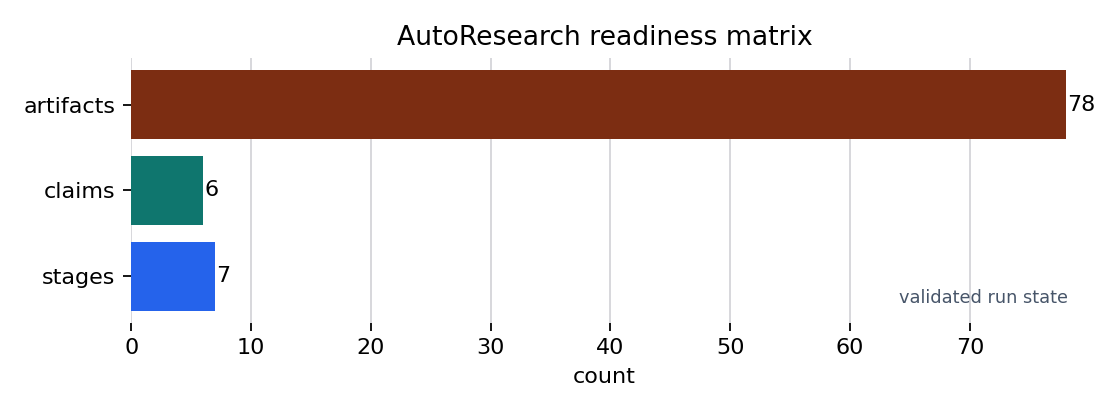
\includegraphics[keepaspectratio,alt={Validated AutoResearch run with 7 stages, 6 supported claims, and 78 required artifacts from output/data/autoresearch\_loop.json; the count summarizes readiness artifacts, not human approval. Generation method: Horizontal count summary from final loop metrics. Registry metadata records the generation method, source artifact, and claim boundary for validation.}]{../figures/autoresearch_stage_matrix.png}}
\caption{Validated AutoResearch run with 7 stages, 6 supported claims,
and 78 required artifacts from output/data/autoresearch\_loop.json; the
count summarizes readiness artifacts, not human approval. Generation
method: Horizontal count summary from final loop metrics. Registry
metadata records the generation method, source artifact, and claim
boundary for validation.}\label{fig:autoresearch_stage_matrix}
\end{figure}

\begin{figure}
\centering
\pandocbounded{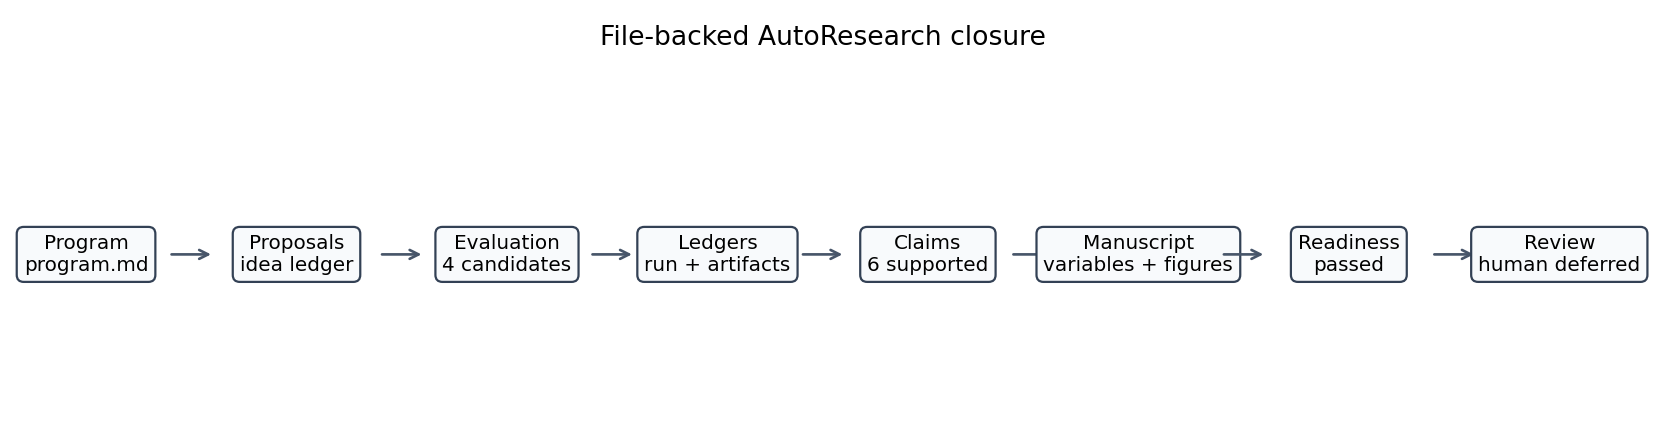
\includegraphics[keepaspectratio,alt={File-backed AutoResearch closure from program through review, with 6 supported claims and readiness passed; review remains a deferred human decision and the provenance path remains inspectable. Generation method: File-backed process-flow diagram from final loop state. Registry metadata records the generation method, source artifact, and claim boundary for validation.}]{../figures/autoresearch_closure_flow.png}}
\caption{File-backed AutoResearch closure from program through review,
with 6 supported claims and readiness passed; review remains a deferred
human decision and the provenance path remains inspectable. Generation
method: File-backed process-flow diagram from final loop state. Registry
metadata records the generation method, source artifact, and claim
boundary for validation.}\label{fig:autoresearch_closure_flow}
\end{figure}

\begin{longtable}[]{@{}
  >{\raggedright\arraybackslash}p{(\linewidth - 4\tabcolsep) * \real{0.3333}}
  >{\raggedright\arraybackslash}p{(\linewidth - 4\tabcolsep) * \real{0.3333}}
  >{\raggedright\arraybackslash}p{(\linewidth - 4\tabcolsep) * \real{0.3333}}@{}}
\caption{Generated artifact manifest from
\protect\breaktt{output/reports/artifact\_manifest.json}.}\label{tbl:autoresearch-loop}\tabularnewline
\toprule\noalign{}
\begin{minipage}[b]{\linewidth}\raggedright
Artifact
\end{minipage} & \begin{minipage}[b]{\linewidth}\raggedright
Role
\end{minipage} & \begin{minipage}[b]{\linewidth}\raggedright
Bytes
\end{minipage} \\
\midrule\noalign{}
\endfirsthead
\toprule\noalign{}
\begin{minipage}[b]{\linewidth}\raggedright
Artifact
\end{minipage} & \begin{minipage}[b]{\linewidth}\raggedright
Role
\end{minipage} & \begin{minipage}[b]{\linewidth}\raggedright
Bytes
\end{minipage} \\
\midrule\noalign{}
\endhead
\bottomrule\noalign{}
\endlastfoot
output/data/autoresearch\_claims.json & Loop artifact & 1766 \\
output/data/autoresearch\_evidence\_overview.json & Evidence registry &
4436 \\
output/data/autoresearch\_integrity\_attestation.json & Security
evidence & 22755 \\
output/data/autoresearch\_inventory\_export.json & Security evidence &
20203 \\
output/data/autoresearch\_loop.json & Loop artifact & 16085 \\
output/data/autoresearch\_phase\_ledger.json & Run or candidate ledger &
3779 \\
output/data/autoresearch\_plan.json & Loop artifact & 17361 \\
output/data/autoresearch\_review\_packet.json & Review packet & 16204 \\
output/data/autoresearch\_schema\_manifest.json & Loop artifact &
7226 \\
output/data/autoresearch\_security\_profile.json & Security evidence &
1537 \\
output/data/autoresearch\_stage\_matrix.csv & Loop artifact & 749 \\
output/data/autoresearch\_supply\_chain\_inventory.json & Security
evidence & 21459 \\
output/data/autoresearch\_threat\_model.json & Security evidence &
6370 \\
output/data/benchmark\_boundary.json & Benchmark grading & 2363 \\
output/data/benchmark\_scores.json & Benchmark grading & 621 \\
output/data/figure\_quality\_report.json & Loop artifact & 16040 \\
output/data/figure\_style.json & Loop artifact & 1117 \\
output/data/idea\_ledger.json & Run or candidate ledger & 5233 \\
output/data/manuscript\_figure\_blocks.json & Manuscript hydration &
13062 \\
output/data/manuscript\_variable\_provenance.json & Manuscript hydration
& 30891 \\
output/data/manuscript\_variables.json & Manuscript hydration & 54968 \\
output/data/ml\_bootstrap\_intervals.json & Loop artifact & 615 \\
output/data/ml\_calibration\_bin\_intervals.json & Loop artifact &
2879 \\
output/data/ml\_calibration\_report.json & Loop artifact & 2201 \\
output/data/ml\_candidate\_intervals.json & Loop artifact & 1577 \\
output/data/ml\_candidate\_ledger.json & Run or candidate ledger &
570872 \\
output/data/ml\_candidate\_rank\_stability.json & Loop artifact &
3135 \\
output/data/ml\_candidate\_selection\_audit.json & Loop artifact &
2145 \\
output/data/ml\_class\_balance.json & Loop artifact & 2393 \\
output/data/ml\_classification\_diagnostics.json & Loop artifact &
4246 \\
output/data/ml\_confusion\_matrix.csv & Loop artifact & 271 \\
output/data/ml\_diagnostic\_boundary.json & Loop artifact & 2064 \\
output/data/ml\_error\_examples.json & Loop artifact & 989 \\
output/data/ml\_paired\_comparison.json & Loop artifact & 470 \\
output/data/ml\_prediction\_records.json & Loop artifact & 989913 \\
output/data/ml\_probability\_diagnostics.json & Loop artifact & 3045 \\
output/data/ml\_robustness\_report.json & Loop artifact & 3758 \\
output/data/ml\_statistical\_summary.json & Loop artifact & 3032 \\
output/data/ml\_task\_results.json & Loop artifact & 703566 \\
output/data/ml\_training\_diagnostics.json & Loop artifact & 2968 \\
output/data/ml\_training\_history.csv & Loop artifact & 6775 \\
output/data/mnist\_task\_config.json & Loop artifact & 3926 \\
output/data/research\_object\_manifest.json & Loop artifact & 20789 \\
output/data/research\_program.json & Loop artifact & 965 \\
output/data/review\_decisions.json & Review packet & 669 \\
output/data/run\_ledger.json & Run or candidate ledger & 328 \\
../figures/autoresearch\_candidate\_lifecycle.png & Generated figure &
28053 \\
../figures/autoresearch\_closure\_flow.png & Generated figure & 40410 \\
../figures/autoresearch\_integrity\_chain.png & Generated figure &
48256 \\
../figures/autoresearch\_security\_control\_matrix.png & Generated
figure & 86574 \\
../figures/ml\_bootstrap\_intervals.png & Generated figure & 21834 \\
../figures/ml\_calibration\_reliability.png & Generated figure &
73889 \\
../figures/ml\_candidate\_rank\_stability.png & Generated figure &
43692 \\
../figures/ml\_candidate\_scores.png & Generated figure & 59953 \\
../figures/ml\_classification\_metrics\_heatmap.png & Generated figure &
55092 \\
../figures/ml\_complexity\_accuracy.png & Generated figure & 35135 \\
../figures/ml\_confusion\_matrix.png & Generated figure & 65820 \\
../figures/ml\_confusion\_pairs.png & Generated figure & 33982 \\
../figures/ml\_generalization\_gap.png & Generated figure & 48512 \\
../figures/ml\_learning\_curves.png & Generated figure & 59258 \\
../figures/ml\_paired\_correctness.png & Generated figure & 43309 \\
../figures/ml\_per\_class\_accuracy.png & Generated figure & 34800 \\
../figures/ml\_probability\_margin\_distribution.png & Generated figure
& 41754 \\
../figures/ml\_probability\_quality.png & Generated figure & 38071 \\
../figures/ml\_robustness\_matrix.png & Generated figure & 51332 \\
../figures/ml\_selective\_accuracy.png & Generated figure & 48274 \\
../figures/ml\_training\_dynamics.png & Generated figure & 51004 \\
../figures/mnist\_class\_balance.png & Generated figure & 27059 \\
../figures/mnist\_error\_examples.png & Generated figure & 28431 \\
../figures/mnist\_subset\_contact\_sheet.png & Generated figure &
23617 \\
output/reports/autoresearch\_evidence\_overview.md & Evidence registry &
1136 \\
output/reports/autoresearch\_loop.json & Loop artifact & 16085 \\
output/reports/autoresearch\_review\_packet.md & Review packet & 912 \\
output/reports/autoresearch\_security\_review.md & Review packet &
1104 \\
output/reports/autoresearch\_summary.md & Loop artifact & 255 \\
output/reports/benchmark\_readiness\_smoke.json & Benchmark grading &
778 \\
output/reports/ml\_benchmark\_score.json & Benchmark grading & 382 \\
output/reports/ml\_experiment\_report.md & Loop artifact & 1687 \\
\end{longtable}

\begin{longtable}[]{@{}
  >{\raggedright\arraybackslash}p{(\linewidth - 6\tabcolsep) * \real{0.2500}}
  >{\raggedright\arraybackslash}p{(\linewidth - 6\tabcolsep) * \real{0.2500}}
  >{\raggedright\arraybackslash}p{(\linewidth - 6\tabcolsep) * \real{0.2500}}
  >{\raggedright\arraybackslash}p{(\linewidth - 6\tabcolsep) * \real{0.2500}}@{}}
\caption{Review-gate decisions from
\protect\breaktt{output/data/review\_decisions.json}.}\label{tbl:review-gates}\tabularnewline
\toprule\noalign{}
\begin{minipage}[b]{\linewidth}\raggedright
Gate
\end{minipage} & \begin{minipage}[b]{\linewidth}\raggedright
Required
\end{minipage} & \begin{minipage}[b]{\linewidth}\raggedright
Decision
\end{minipage} & \begin{minipage}[b]{\linewidth}\raggedright
Rationale
\end{minipage} \\
\midrule\noalign{}
\endfirsthead
\toprule\noalign{}
\begin{minipage}[b]{\linewidth}\raggedright
Gate
\end{minipage} & \begin{minipage}[b]{\linewidth}\raggedright
Required
\end{minipage} & \begin{minipage}[b]{\linewidth}\raggedright
Decision
\end{minipage} & \begin{minipage}[b]{\linewidth}\raggedright
Rationale
\end{minipage} \\
\midrule\noalign{}
\endhead
\bottomrule\noalign{}
\endlastfoot
proposal\_review & True & deferred & Decision is read from
human\_review.yaml when present; generated readiness is not approval. \\
evidence\_review & True & deferred & Decision is read from
human\_review.yaml when present; generated readiness is not approval. \\
\end{longtable}

\begin{longtable}[]{@{}
  >{\raggedright\arraybackslash}p{(\linewidth - 6\tabcolsep) * \real{0.2500}}
  >{\raggedright\arraybackslash}p{(\linewidth - 6\tabcolsep) * \real{0.2500}}
  >{\raggedright\arraybackslash}p{(\linewidth - 6\tabcolsep) * \real{0.2500}}
  >{\raggedright\arraybackslash}p{(\linewidth - 6\tabcolsep) * \real{0.2500}}@{}}
\caption{Benchmark grading table from
\protect\breaktt{output/data/benchmark\_scores.json}.}\label{tbl:benchmark-scores}\tabularnewline
\toprule\noalign{}
\begin{minipage}[b]{\linewidth}\raggedright
Benchmark task
\end{minipage} & \begin{minipage}[b]{\linewidth}\raggedright
Status
\end{minipage} & \begin{minipage}[b]{\linewidth}\raggedright
Score
\end{minipage} & \begin{minipage}[b]{\linewidth}\raggedright
Grading output
\end{minipage} \\
\midrule\noalign{}
\endfirsthead
\toprule\noalign{}
\begin{minipage}[b]{\linewidth}\raggedright
Benchmark task
\end{minipage} & \begin{minipage}[b]{\linewidth}\raggedright
Status
\end{minipage} & \begin{minipage}[b]{\linewidth}\raggedright
Score
\end{minipage} & \begin{minipage}[b]{\linewidth}\raggedright
Grading output
\end{minipage} \\
\midrule\noalign{}
\endhead
\bottomrule\noalign{}
\endlastfoot
readiness-smoke & graded & 1 &
output/reports/benchmark\_readiness\_smoke.json \\
ml-loop-score & graded & 1 & output/reports/ml\_benchmark\_score.json \\
\end{longtable}

\begin{longtable}[]{@{}
  >{\raggedright\arraybackslash}p{(\linewidth - 8\tabcolsep) * \real{0.2000}}
  >{\raggedright\arraybackslash}p{(\linewidth - 8\tabcolsep) * \real{0.2000}}
  >{\raggedright\arraybackslash}p{(\linewidth - 8\tabcolsep) * \real{0.2000}}
  >{\raggedright\arraybackslash}p{(\linewidth - 8\tabcolsep) * \real{0.2000}}
  >{\raggedright\arraybackslash}p{(\linewidth - 8\tabcolsep) * \real{0.2000}}@{}}
\caption{Deterministic phase ledger from
\protect\breaktt{output/data/autoresearch\_phase\_ledger.json};
settlement order is not an autonomy
claim.}\label{tbl:phase-ledger}\tabularnewline
\toprule\noalign{}
\begin{minipage}[b]{\linewidth}\raggedright
Phase
\end{minipage} & \begin{minipage}[b]{\linewidth}\raggedright
Order
\end{minipage} & \begin{minipage}[b]{\linewidth}\raggedright
Group
\end{minipage} & \begin{minipage}[b]{\linewidth}\raggedright
Observed artifacts
\end{minipage} & \begin{minipage}[b]{\linewidth}\raggedright
Description
\end{minipage} \\
\midrule\noalign{}
\endfirsthead
\toprule\noalign{}
\begin{minipage}[b]{\linewidth}\raggedright
Phase
\end{minipage} & \begin{minipage}[b]{\linewidth}\raggedright
Order
\end{minipage} & \begin{minipage}[b]{\linewidth}\raggedright
Group
\end{minipage} & \begin{minipage}[b]{\linewidth}\raggedright
Observed artifacts
\end{minipage} & \begin{minipage}[b]{\linewidth}\raggedright
Description
\end{minipage} \\
\midrule\noalign{}
\endhead
\bottomrule\noalign{}
\endlastfoot
intrinsic readiness & 1 & readiness & 3 & validate configured
project-intrinsic contracts \\
core artifacts & 2 & loop & 0 & write plan, stage matrix, and
provisional loop outputs \\
evidence registry & 3 & evidence & 2 & write local evidence registry \\
ml task & 4 & ml & 54 & run fixed-seed bounded candidate evaluation \\
method contract & 5 & governance & 3 & write program, idea, run, review,
and benchmark ledgers \\
provisional payloads & 6 & settlement & 12 & refresh loop payloads
before extrinsic validation \\
security artifacts & 7 & security & 10 & write local security and
integrity evidence \\
final visuals & 8 & figures & 54 & write final registry-backed
figures \\
manuscript hydration & 9 & manuscript & 9 & write variables, provenance,
and figure blocks \\
readiness manifest & 10 & settlement & 12 & refresh checksum manifest
before extrinsic validation \\
schema manifest & 11 & schema & 2 & write generated JSON schema-version
manifest \\
research object manifest & 12 & packaging & 2 & write local
research-object manifest \\
extrinsic readiness & 13 & readiness & 3 & validate generated artifacts
and extrinsic contracts \\
final schema manifest & 14 & schema & 2 & refresh schema manifest after
final payload updates \\
final research object manifest & 15 & packaging & 2 & refresh local
research-object manifest \\
artifact manifest & 16 & settlement & 12 & write final artifact checksum
manifest \\
\end{longtable}

\begin{longtable}[]{@{}
  >{\raggedright\arraybackslash}p{(\linewidth - 8\tabcolsep) * \real{0.2000}}
  >{\raggedright\arraybackslash}p{(\linewidth - 8\tabcolsep) * \real{0.2000}}
  >{\raggedright\arraybackslash}p{(\linewidth - 8\tabcolsep) * \real{0.2000}}
  >{\raggedright\arraybackslash}p{(\linewidth - 8\tabcolsep) * \real{0.2000}}
  >{\raggedright\arraybackslash}p{(\linewidth - 8\tabcolsep) * \real{0.2000}}@{}}
\caption{Figure-quality checks from
\protect\breaktt{output/data/figure\_quality\_report.json}; 25 registered
figure(s) were checked.}\label{tbl:figure-quality}\tabularnewline
\toprule\noalign{}
\begin{minipage}[b]{\linewidth}\raggedright
Figure
\end{minipage} & \begin{minipage}[b]{\linewidth}\raggedright
Pixels
\end{minipage} & \begin{minipage}[b]{\linewidth}\raggedright
Variance
\end{minipage} & \begin{minipage}[b]{\linewidth}\raggedright
Source exists
\end{minipage} & \begin{minipage}[b]{\linewidth}\raggedright
Nonblank
\end{minipage} \\
\midrule\noalign{}
\endfirsthead
\toprule\noalign{}
\begin{minipage}[b]{\linewidth}\raggedright
Figure
\end{minipage} & \begin{minipage}[b]{\linewidth}\raggedright
Pixels
\end{minipage} & \begin{minipage}[b]{\linewidth}\raggedright
Variance
\end{minipage} & \begin{minipage}[b]{\linewidth}\raggedright
Source exists
\end{minipage} & \begin{minipage}[b]{\linewidth}\raggedright
Nonblank
\end{minipage} \\
\midrule\noalign{}
\endhead
\bottomrule\noalign{}
\endlastfoot
fig:autoresearch\_candidate\_lifecycle & 1184x480 & 0.083 & True &
True \\
fig:autoresearch\_closure\_flow & 1664x448 & 0.015 & True & True \\
fig:autoresearch\_integrity\_chain & 1440x734 & 0.040 & True & True \\
fig:autoresearch\_security\_control\_matrix & 1470x734 & 0.014 & True &
True \\
fig:autoresearch\_stage\_matrix & 1120x416 & 0.080 & True & True \\
fig:ml\_bootstrap\_intervals & 1152x448 & 0.009 & True & True \\
fig:ml\_calibration\_reliability & 1152x832 & 0.015 & True & True \\
fig:ml\_candidate\_rank\_stability & 1408x608 & 0.053 & True & True \\
fig:ml\_candidate\_scores & 1376x688 & 0.013 & True & True \\
fig:ml\_classification\_metrics\_heatmap & 928x832 & 0.092 & True &
True \\
fig:ml\_complexity\_accuracy & 1120x608 & 0.010 & True & True \\
fig:ml\_confusion\_matrix & 896x768 & 0.046 & True & True \\
fig:ml\_confusion\_pairs & 1152x576 & 0.129 & True & True \\
fig:ml\_generalization\_gap & 1184x864 & 0.059 & True & True \\
fig:ml\_learning\_curves & 1216x608 & 0.018 & True & True \\
fig:ml\_paired\_correctness & 768x672 & 0.075 & True & True \\
fig:ml\_per\_class\_accuracy & 1152x512 & 0.098 & True & True \\
fig:ml\_probability\_margin\_distribution & 1184x864 & 0.024 & True &
True \\
fig:ml\_probability\_quality & 1344x608 & 0.046 & True & True \\
fig:ml\_robustness\_matrix & 1280x608 & 0.073 & True & True \\
fig:ml\_selective\_accuracy & 1088x608 & 0.016 & True & True \\
fig:ml\_training\_dynamics & 1408x608 & 0.072 & True & True \\
fig:mnist\_class\_balance & 1216x544 & 0.071 & True & True \\
fig:mnist\_error\_examples & 1280x734 & 0.234 & True & True \\
fig:mnist\_subset\_contact\_sheet & 1216x544 & 0.228 & True & True \\
\end{longtable}

\subsection{Security Readiness And Integrity
Evidence}\label{sec:security-readiness-integrity}

The local security profile reports attestation status \texttt{passed}
after checking \texttt{80} file record(s), with \texttt{0} missing
record(s) and \texttt{0} checksum mismatch(es). The inventory contains
\texttt{14} input record(s) and \texttt{69} generated-artifact
record(s). The integrity-chain figure is
fig.~\ref{fig:autoresearch_integrity_chain}. These values support local
artifact-integrity claims only; they do not claim external signing,
production SLSA compliance, or runtime security monitoring.

\begin{figure}
\centering
\pandocbounded{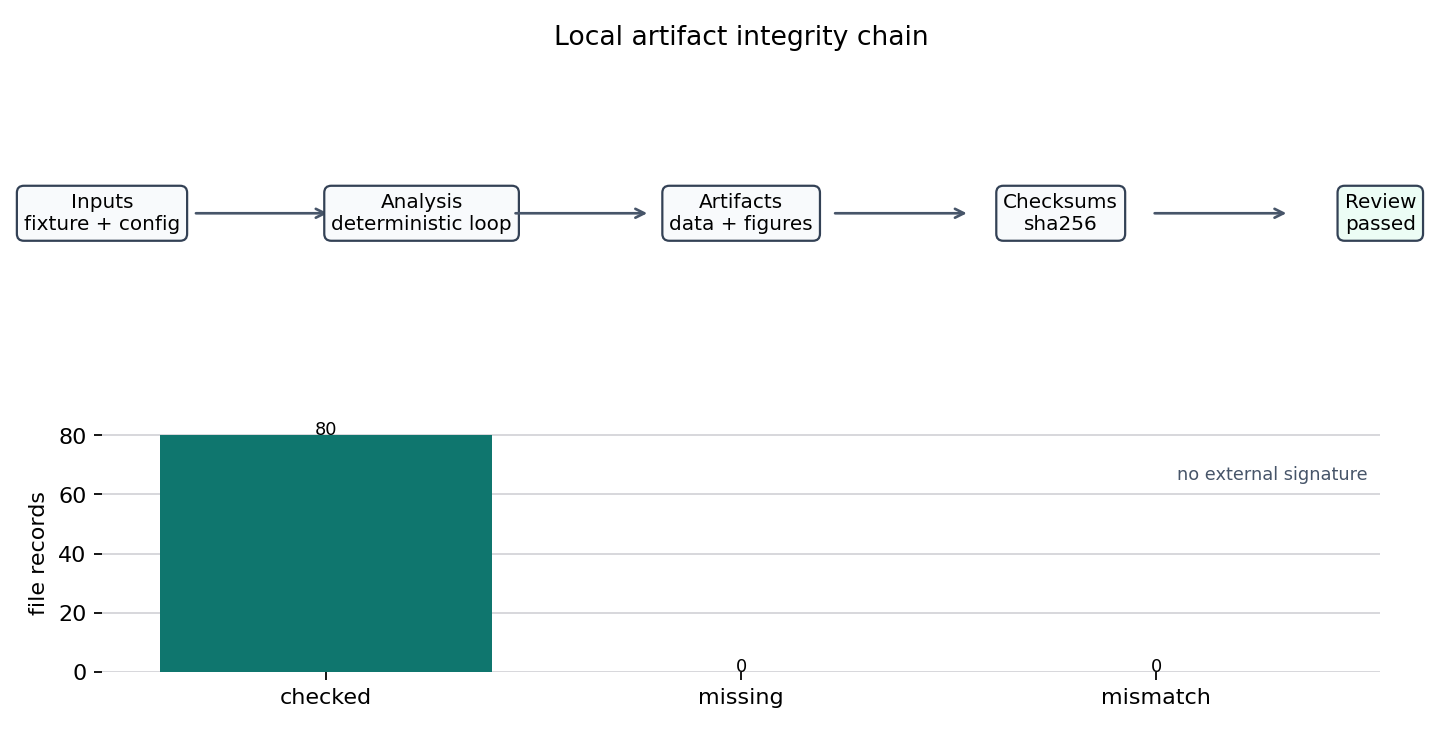
\includegraphics[keepaspectratio,alt={Local integrity chain from output/data/autoresearch\_integrity\_attestation.json; checksums summarize the observed run artifacts and remain unsigned local evidence. Generation method: Local checksum attestation chain with checked, missing, and mismatch counts. Registry metadata records the generation method, source artifact, and claim boundary for validation.}]{../figures/autoresearch_integrity_chain.png}}
\caption{Local integrity chain from
output/data/autoresearch\_integrity\_attestation.json; checksums
summarize the observed run artifacts and remain unsigned local evidence.
Generation method: Local checksum attestation chain with checked,
missing, and mismatch counts. Registry metadata records the generation
method, source artifact, and claim boundary for
validation.}\label{fig:autoresearch_integrity_chain}
\end{figure}

\begin{longtable}[]{@{}ll@{}}
\caption{Integrity-attestation summary from
\protect\breaktt{output/data/autoresearch\_integrity\_attestation.json}.}\label{tbl:security-integrity}\tabularnewline
\toprule\noalign{}
Integrity field & Value \\
\midrule\noalign{}
\endfirsthead
\toprule\noalign{}
Integrity field & Value \\
\midrule\noalign{}
\endhead
\bottomrule\noalign{}
\endlastfoot
status & passed \\
algorithm & sha256 \\
checked files & 80 \\
missing files & 0 \\
checksum mismatches & 0 \\
external signature & False \\
\end{longtable}

\subsection{Manuscript Hydration
Provenance}\label{sec:manuscript-hydration-provenance}

The final run supports \texttt{6} manuscript-facing claim(s) and checks
\texttt{78} required artifact(s). The rendered manuscript uses injected
variables from generated data payloads, so the abstract and results
track the latest analysis run rather than hard-coded counts. The final
readiness status is \texttt{passed}; generated review decisions are
recorded as deferred for human review rather than as self-approval.

\begin{longtable}[]{@{}ll@{}}
\caption{Variable provenance summary from
\protect\breaktt{output/data/manuscript\_variable\_provenance.json}.}\label{tbl:variable-provenance}\tabularnewline
\toprule\noalign{}
Source artifact & Injected variables or fragments \\
\midrule\noalign{}
\endfirsthead
\toprule\noalign{}
Source artifact & Injected variables or fragments \\
\midrule\noalign{}
\endhead
\bottomrule\noalign{}
\endlastfoot
output/data/autoresearch\_integrity\_attestation.json & 5 \\
output/data/autoresearch\_loop.json & 57 \\
output/data/autoresearch\_phase\_ledger.json & 2 \\
output/data/autoresearch\_schema\_manifest.json & 1 \\
output/data/autoresearch\_security\_profile.json & 6 \\
output/data/autoresearch\_supply\_chain\_inventory.json & 3 \\
output/data/autoresearch\_threat\_model.json & 4 \\
output/data/benchmark\_scores.json & 1 \\
output/data/figure\_quality\_report.json & 3 \\
output/data/manuscript\_variable\_provenance.json & 1 \\
output/data/ml\_bootstrap\_intervals.json & 3 \\
output/data/ml\_calibration\_bin\_intervals.json & 1 \\
output/data/ml\_calibration\_report.json & 3 \\
output/data/ml\_candidate\_intervals.json & 1 \\
output/data/ml\_candidate\_ledger.json & 1 \\
output/data/ml\_candidate\_rank\_stability.json & 3 \\
output/data/ml\_candidate\_selection\_audit.json & 1 \\
output/data/ml\_class\_balance.json & 3 \\
output/data/ml\_classification\_diagnostics.json & 5 \\
output/data/ml\_diagnostic\_boundary.json & 1 \\
output/data/ml\_paired\_comparison.json & 3 \\
output/data/ml\_probability\_diagnostics.json & 4 \\
output/data/ml\_robustness\_report.json & 2 \\
output/data/ml\_statistical\_summary.json & 9 \\
output/data/ml\_task\_results.json & 39 \\
output/data/ml\_training\_diagnostics.json & 7 \\
output/data/research\_object\_manifest.json & 2 \\
output/data/review\_decisions.json & 1 \\
../figures/figure\_registry.json & 51 \\
output/reports/artifact\_manifest.json & 1 \\
\end{longtable}

\newpage

\section{Conclusion}\label{sec:conclusion}

\breaktt{template\_autoresearch\_project} shows how a tractable
AutoResearch task can be represented as reproducible template
infrastructure. The
\breaktt{small\ MNIST\ neural-network\ classification} experiment is
small by design, but it exercises the method surfaces that matter for a
public default: a declared research program, local input-data
provenance, bounded candidate families
(\breaktt{MLP,\ nearest-centroid,\ softmax\ regression,\ tiny\ patch-attention}),
objective scoring, budget and cost ledgers, evidence-linked claims,
generated figures, benchmark grading, manuscript-variable hydration,
loop-settlement ledgers, figure-quality checks, validation, local
integrity attestation (\texttt{passed}), and human review gates.

The broader field is converging across five related trends. Autoresearch
systems seek end-to-end automation of ideation, experiment execution,
writing, and review. Autoformalization pushes informal claims toward
machine-checkable representations. ML-for-ML systems use search,
evaluation, and evolutionary code loops to improve algorithms. Agentic
science composes retrieval, planning, experimentation, and communication
into higher-autonomy workflows. Structured knowledge synthesis supplies
the substrate that all of those systems need: source-linked artifacts,
knowledge graphs, tensors, vector spaces, and uncertainty-aware memories
that can be navigated without losing provenance.

This exemplar makes a deliberately narrower contribution. It does not
mine the live literature, construct a Conceptual Nexus Model, search for
Lean proofs, mutate arbitrary code, coordinate external agents, or
approve its own paper. Instead it demonstrates governance infrastructure
for automated research workflows: every important claim is hydrated from
run artifacts, every generated figure is registry-bound and locally
checked for source and pixel integrity, every budget and candidate
decision is recorded, and review state remains outside generated
self-approval. The security layer adds local inventory and checksum
evidence while keeping external signing and production deployment claims
out of scope.

The durable product is therefore not only the \texttt{MNIST} metric. It
is a reproducible research process whose data, claims, captions,
figures, review gates, and manuscript variables can be reviewed, rerun,
and extended. As more ambitious automated-science systems mature, this
kind of offline, deterministic, evidence-governed baseline remains
useful because it preserves the part of scientific automation that
should not be optional: inspectable provenance, explicit limits, and
human-governed publication judgment.

\newpage

\section{References}\label{references}

References are managed in \texttt{references.bib}.

\newpage



\clearpage

\bibliography{references}
% transmission-end-bookend
\clearpage
\thispagestyle{empty}
\setlength{\parskip}{0pt}
\setlength{\itemsep}{0pt}
\begin{samepage}
\scriptsize

\section*{END OF TRANSMISSION}\label{end-of-transmission}

\textbf{Release:} v0.3.2 \texorpdfstring{\ensuremath{\cdot}}{.} DOI \breaktt{10.5281/zenodo.20417016} \texorpdfstring{\ensuremath{\cdot}}{.}
SHA-256 \texttt{e07b62850a19…} \texorpdfstring{\ensuremath{\cdot}}{.} pairing complete

\begin{figure}
\centering
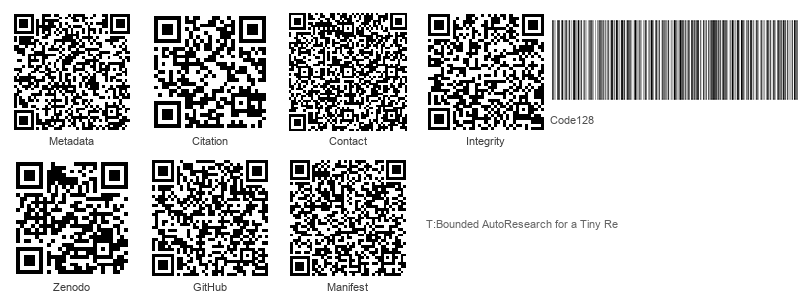
\includegraphics[width=0.88\linewidth,height=0.50\textheight,keepaspectratio,alt={Integrity QR strip}]{../figures/transmission_integrity_strip.png}
\caption{Integrity QR strip}
\end{figure}

\textbf{Prior:} \texttt{v0.3.1} \texorpdfstring{\ensuremath{\cdot}}{.} \breaktt{10.5281/zenodo.20417016} \texorpdfstring{\ensuremath{\cdot}}{.}
\texttt{537dd8a6…}

\end{samepage}

\end{document}
